%                                                                 aa.dem
% AA vers. 9.1, LaTeX class for Astronomy & Astrophysics
% demonstration file
%                                                       (c) EDP Sciences
%-----------------------------------------------------------------------
%
% \documentclass[referee]{aa} % for a referee version
%\documentclass[onecolumn]{aa} % for a paper on 1 column  
%\documentclass[longauth]{aa} % for the long lists of affiliations 
%\documentclass[letter]{aa} % for the letters 
%\documentclass[bibyear]{aa} % if the references are not structured 
%                              according to the author-year natbib style

%

\documentclass{aa}  

%
\usepackage{graphicx}
\usepackage{amsmath,amsfonts,amssymb}
\usepackage{natbib}


%%%%%%%%%%%%%%%%%%%%%%%%%%%%%%%%%%%%%%%%
\usepackage{txfonts}
\usepackage{xcolor}

\usepackage{blindtext}
%%%%%%%%%%%%%%%%%%%%%%%%%%%%%%%%%%%%%%%%
% \usepackage[options]{hyperref}
% To add links in your PDF file, use the package "hyperref"
% with options according to your LaTeX or PDFLaTeX drivers.
\usepackage{float}
%\usepackage{stfloats}
\usepackage{dblfloatfix}
\usepackage{afterpage}
\usepackage{ifthen}
\usepackage[morefloats=12]{morefloats}

\usepackage{placeins}
\usepackage{multicol}
\usepackage[export]{adjustbox}\usepackage[breaklinks,colorlinks,citecolor=blue]{hyperref}
\bibpunct{(}{)}{;}{a}{}{,}
\usepackage[switch]{lineno}
\definecolor{linkcolor}{rgb}{0.6,0,0}
\definecolor{citecolor}{rgb}{0,0,0.75}
\definecolor{urlcolor}{rgb}{0.12,0.46,0.7}
%\usepackage[breaklinks, colorlinks, urlcolor=urlcolor,linkcolor=linkcolor,citecolor=citecolor,pdfencoding=auto]{hyperref}
\hypersetup{linktocpage}
\usepackage{bold-extra}
\usepackage{tabularx, booktabs}
\usepackage{amsmath}

%Planck style file, to be used with A&A style to produce Planck papers for publication.
%
% version 28 September 2010 --- useful macros --- CRL
% version 17 October 2010   --- first cut at important instrument values, from Daniele Mennella and
%                               Francois Bouchet, 13 October 2010 --- CRL
% version 18 October 2010   --- LFI FWHM changed to one value per feed, rather than M & S separately
%                               LFI FWHM uncertainties added for individual feeds.  Corrections made
%                               to LFI values. --- Andrea Zacchei
% version 24 October 2010   --- added to and corrected definitions.  No changes made to instrument
%                               quantities. --- CRL 
% version 31 October 2010   --- added definition of \muKHz. --- CRL
%
% version 15 November 2010  --- fixed conflict with aa.cls in definition of \endtable
%                               by naming the command below "\endPlancktable".  See section
%                               13.16 of the Style Guide.
%
% version 06 December 2010  --- Set up names with and without units.
%                               Add \allearlypapers command to ensure that all early papers are
%                               included in the reference list.
%                               Define macro for the name of the 4He JT cooler.
%
% version 07 December 2010  --- removed extraneous "planck2011-1.2" entry in \allearlypapers
%
% version 12 December 2010  --- added \endPlancktablewide command to set tablenotes to the full
%                               page width in the \begin{table*}...\end{table*} environment when
%                               the ``twocolumn'' option is specified in the \documentclass command.
%                               (It would be more elegant to extract the appropriate width from the
%                               aa.cls system at the time of execution, but that is buried more
%                               deeply in the system than I investigated.)
%
% version 05 January 2011   --- added unit \MJysr.  HFI performance values updated per FRB email
%                               01/05/2011 02:38-0800, and Brendan Crill email 01/05/2011 18:08 -0800.
%
% version 06 January 2011   --- changed \scriptscriptstyle primes to \scriptstyle, to better match the
%                               tx fonts used by A&A.
%
% version 07 January 2011   --- modified \allearlypapers to correspond with final early paper list.  
%                               Fixed 545 GHz center frequency.
%
% version 07 January 2011b  --- changed LFI white-noise sensitivity numbers to correct problem with units
%
% version 05 July 2011      --- added \Msol and \Lsol to get the symbols for solar mass and luminosity.
%                               Deleted previous definitions of \solar and \sol, which were equivalent
%                               to the new \Msol.
%
% version 16 August 2011    --- changed comments on \endPlancktable and \endPlancktablewide for clarity
%
% version 11 September 2011 --- changed definition of \tablenote to make footnote labels italic, as per A\&A
%
% version 26 April 2011     --- changed definition of \Planck to agree with what is said in the Style Guide (!)
%
% version 04 Dec 2013       --- included 2013 results references
%
% version 17 Jan 2014       --- included fix to bibtex file v4.3, i.e. \providecommand{\sorthelp}[1]{}
%
% version 26 Jul 2014       --- fixed incompatibility problem with aa.cls v8.0 and v8.2.  v8.2 should now be used
%                               for all Planck papers.
%                           --- fixed problem in definition of "\all2013resultspapers" that introduced a blanck
%                               into the reference to p06b.
%                           --- removed all the parameter definition stuff at the end.  We weren't using it, and
%                               it took up a lot of space.
%
% version 28 Jan 2015       --- added "\alltwentyfiftennresultspapers" and corrected "\all2013resultspapers" to
%                               "\all20thirteenresultspapers",
%
% Usage:  after the \documentclass[traditabstract]{aa} command in the La\TeX\ input file,
%         add this command:      \input Planck.tex


\def\setsymbol#1#2{\expandafter\def\csname #1\endcsname{#2}}
\def\getsymbol#1{\csname #1\endcsname}

%-----------------------------------------------------------------------
% Planck
%-----------------------------------------------------------------------
\def\Planck{\textit{Planck}}

%-----------------------------------------------------------------------
% The Planck Helium-4 JT cooler
%-----------------------------------------------------------------------
\def\HeJT{$^4$He-JT}

%-----------------------------------------------------------------------
% To include all Planck Early Results papers in the reference lists
%-----------------------------------------------------------------------
\def\allearlypapers{\nocite{planck2011-1.1, planck2011-1.3, planck2011-1.4, planck2011-1.5, planck2011-1.6, planck2011-1.7, planck2011-1.10, planck2011-1.10sup, planck2011-5.1a, planck2011-5.1b, planck2011-5.2a, planck2011-5.2b, planck2011-5.2c, planck2011-6.1, planck2011-6.2, planck2011-6.3a, planck2011-6.4a, planck2011-6.4b, planck2011-6.6, planck2011-7.0, planck2011-7.2, planck2011-7.3, planck2011-7.7a, planck2011-7.7b, planck2011-7.12, planck2011-7.13}}

%-----------------------------------------------------------------------
% To include all Planck 2013 Results papers in the reference lists
%-----------------------------------------------------------------------
\def\alltwentythirteenresultspapers{\nocite{planck2013-p01, planck2013-p02, planck2013-p02a, planck2013-p02d, planck2013-p02b, planck2013-p03, planck2013-p03c, planck2013-p03f, planck2013-p03d, planck2013-p03e, planck2013-p01a, planck2013-p06, planck2013-p03a, planck2013-pip88, planck2013-p08, planck2013-p11, planck2013-p12, planck2013-p13, planck2013-p14, planck2013-p15, planck2013-p05b, planck2013-p17, planck2013-p09, planck2013-p09a, planck2013-p20, planck2013-p19, planck2013-pipaberration, planck2013-p05, planck2013-p05a, planck2013-pip56, planck2013-p06b, planck2013-p01a}}

%-----------------------------------------------------------------------
% To include all Planck 2015 Results papers in the reference lists
%-----------------------------------------------------------------------
\def\alltwentyfifteenresultspapers{\nocite{planck2014-a01, planck2014-a03, planck2014-a04, planck2014-a05, planck2014-a06, planck2014-a07, planck2014-a08, planck2014-a09, planck2014-a11, planck2014-a12, planck2014-a13, planck2014-a14, planck2014-a15, planck2014-a16, planck2014-a17, planck2014-a18, planck2014-a19, planck2014-a20, planck2014-a22, planck2014-a24, planck2014-a26, planck2014-a28, planck2014-a29, planck2014-a30, planck2014-a31, planck2014-a35, planck2014-a36, planck2014-a37, planck2014-ES}}

%-----------------------------------------------------------------------
% Tables
%-----------------------------------------------------------------------
\newbox\tablebox    \newdimen\tablewidth
\def\leaderfil{\leaders\hbox to 5pt{\hss.\hss}\hfil}
%
% use the following definition of \endPlancktable for ApJ style notes to tables, set to the 
%         width of the table
% \def\endPlancktable{\tablewidth=\wd\tablebox 
%
% use the following definitions of \endPlancktable and \endPlancktablewide for A&A style notes 
% set to one-column  or full-page width, respectively
\def\endPlancktable{\tablewidth=\columnwidth 
    $$\hss\copy\tablebox\hss$$
    \vskip-\lastskip\vskip -2pt}
\def\endPlancktablewide{\tablewidth=\textwidth 
    $$\hss\copy\tablebox\hss$$
    \vskip-\lastskip\vskip -2pt}
\def\tablenote#1 #2\par{\begingroup \parindent=0.8em
    \abovedisplayshortskip=0pt\belowdisplayshortskip=0pt
    \noindent
    $$\hss\vbox{\hsize\tablewidth \hangindent=\parindent \hangafter=1 \noindent
    \hbox to \parindent{$^#1$\hss}\strut#2\strut\par}\hss$$
    \endgroup}
\def\doubleline{\vskip 3pt\hrule \vskip 1.5pt \hrule \vskip 5pt}

%-----------------------------------------------------------------------
% useful macros
%-----------------------------------------------------------------------
%
\def\L2{\ifmmode L_2\else $L_2$\fi}
%
\def\dtt{\Delta T/T}
\def\DeltaT{\ifmmode \Delta T\else $\Delta T$\fi}
\def\deltat{\ifmmode \Delta t\else $\Delta t$\fi}
\def\fknee{\ifmmode f_{\rm knee}\else $f_{\rm knee}$\fi}
\def\Fmax{\ifmmode F_{\rm max}\else $F_{\rm max}$\fi}
%
\def\solar{\ifmmode{\rm M}_{\mathord\odot}\else${\rm M}_{\mathord\odot}$\fi}
\def\Msolar{\ifmmode{\rm M}_{\mathord\odot}\else${\rm M}_{\mathord\odot}$\fi}
\def\Lsolar{\ifmmode{\rm L}_{\mathord\odot}\else${\rm L}_{\mathord\odot}$\fi}
%
\def\inv{\ifmmode^{-1}\else$^{-1}$\fi}
\def\mo{\ifmmode^{-1}\else$^{-1}$\fi}
\def\sup#1{\ifmmode ^{\rm #1}\else $^{\rm #1}$\fi}
\def\expo#1{\ifmmode \times 10^{#1}\else $\times 10^{#1}$\fi}
%
\def\,{\thinspace}
\def\lsim{\mathrel{\raise .4ex\hbox{\rlap{$<$}\lower 1.2ex\hbox{$\sim$}}}}
\def\gsim{\mathrel{\raise .4ex\hbox{\rlap{$>$}\lower 1.2ex\hbox{$\sim$}}}}
\let\lea=\lsim
\let\gea=\gsim
\def\simprop{\mathrel{\raise .4ex\hbox{\rlap{$\propto$}\lower 1.2ex\hbox{$\sim$}}}}
%
\def\deg{\ifmmode^\circ\else$^\circ$\fi}
\def\pdeg{\ifmmode $\setbox0=\hbox{$^{\circ}$}\rlap{\hskip.11\wd0 .}$^{\circ}
          \else \setbox0=\hbox{$^{\circ}$}\rlap{\hskip.11\wd0 .}$^{\circ}$\fi}
\def\arcs{\ifmmode {^{\scriptstyle\prime\prime}}
          \else $^{\scriptstyle\prime\prime}$\fi}
\def\arcm{\ifmmode {^{\scriptstyle\prime}}
          \else $^{\scriptstyle\prime}$\fi}
\newdimen\sa  \newdimen\sb
\def\parcs{\sa=.07em \sb=.03em
     \ifmmode \hbox{\rlap{.}}^{\scriptstyle\prime\kern -\sb\prime}\hbox{\kern -\sa}
     \else \rlap{.}$^{\scriptstyle\prime\kern -\sb\prime}$\kern -\sa\fi}
\def\parcm{\sa=.08em \sb=.03em
     \ifmmode \hbox{\rlap{.}\kern\sa}^{\scriptstyle\prime}\hbox{\kern-\sb}
     \else \rlap{.}\kern\sa$^{\scriptstyle\prime}$\kern-\sb\fi}
%
\def\ra[#1 #2 #3.#4]{#1\sup{h}#2\sup{m}#3\sup{s}\llap.#4}
\def\dec[#1 #2 #3.#4]{#1\deg#2\arcm#3\arcs\llap.#4}
\def\deco[#1 #2 #3]{#1\deg#2\arcm#3\arcs}
\def\rra[#1 #2]{#1\sup{h}#2\sup{m}}
%
\def\page{\vfill\eject}
\def\dots{\relax\ifmmode \ldots\else $\ldots$\fi}
%
%-----------------------------------------------------------------------
% units
%-----------------------------------------------------------------------
%
\def\WHzsr{\ifmmode $W\,Hz\mo\,sr\mo$\else W\,Hz\mo\,sr\mo\fi}
\def\mHz{\ifmmode $\,mHz$\else \,mHz\fi}
\def\GHz{\ifmmode $\,GHz$\else \,GHz\fi}
\def\mKs{\ifmmode $\,mK\,s$^{1/2}\else \,mK\,s$^{1/2}$\fi}
\def\muKs{\ifmmode \,\mu$K\,s$^{1/2}\else \,$\mu$K\,s$^{1/2}$\fi}
\def\muKRJs{\ifmmode \,\mu$K$_{\rm RJ}$\,s$^{1/2}\else \,$\mu$K$_{\rm RJ}$\,s$^{1/2}$\fi}
\def\muKHz{\ifmmode \,\mu$K\,Hz$^{-1/2}\else \,$\mu$K\,Hz$^{-1/2}$\fi}
\def\MJysr{\ifmmode \,$MJy\,sr\mo$\else \,MJy\,sr\mo\fi}
\def\MJysrmK{\ifmmode \,$MJy\,sr\mo$\,mK$_{\rm CMB}\mo\else \,MJy\,sr\mo\,mK$_{\rm CMB}\mo$\fi}
\def\microns{\ifmmode \,\mu$m$\else \,$\mu$m\fi}
\def\micron{\microns}
\def\muK{\ifmmode \,\mu$K$\else \,$\mu$\hbox{K}\fi}
\def\microK{\ifmmode \,\mu$K$\else \,$\mu$\hbox{K}\fi}
\def\muW{\ifmmode \,\mu$W$\else \,$\mu$\hbox{W}\fi}
\def\kms{\ifmmode $\,km\,s$^{-1}\else \,km\,s$^{-1}$\fi}
\def\kmsMpc{\ifmmode $\,\kms\,Mpc\mo$\else \,\kms\,Mpc\mo\fi}
%
%
%----------------------------------------------------------------------
% set up machinery to list Planck papers in roman numeral order.
%----------------------------------------------------------------------

\providecommand{\sorthelp}[1]{}


\newcommand{\phm}{\phantom{-}}
\newcommand{\dv}[0]{\vec{d}}
\renewcommand{\t}[0]{\vec{t}}
\newcommand{\A}[0]{\tens{A}}
\newcommand{\B}[0]{\mathrm{B}}
\newcommand{\Y}[0]{\tens{Y}}
\newcommand{\n}[0]{\vec{n}}
\newcommand{\red}[0]{\color{red}}
\newcommand{\green}[0]{\color{green}}
\newcommand{\s}[0]{\vec{s}}
\renewcommand{\a}[0]{\vec{a}}
\newcommand{\m}[0]{\vec{m}}
\newcommand{\bv}[0]{\vec{b}}
\newcommand{\f}[0]{\vec{f}}
\newcommand{\F}[0]{\tens{F}}
\newcommand{\T}[0]{\tens{T}}
\newcommand{\Cp}[0]{\tens{C}}
\renewcommand{\L}[0]{\tens{L}}
\newcommand{\g}[0]{\vec{g}}
\newcommand{\N}[0]{\tens{N}}
\newcommand{\M}[0]{\tens{M}}
\newcommand{\iN}[0]{\tens{N}^{-1}}
\newcommand{\iM}[0]{\tens{M}^{-1}}
\newcommand{\w}[0]{\vec{w}}
\renewcommand{\S}[0]{\tens{S}}
\renewcommand{\r}[0]{\vec{r}}
\renewcommand{\u}[0]{\vec{u}}
\newcommand{\q}[0]{\vec{q}}
\renewcommand{\v}[0]{\vec{v}}
\renewcommand{\P}[0]{\tens{P}}
\newcommand{\dt}[0]{d_t}
\newcommand{\di}[0]{d_i}
\newcommand{\nt}[0]{n_t}
\newcommand{\st}[0]{s_t}
\newcommand{\mt}[0]{m_t}
\newcommand{\ft}[0]{f_t}
\newcommand{\Te}[0]{T_{\rm e}}
\newcommand{\EM}[0]{\rm EM}
\newcommand{\hi}{\ensuremath{\mathsc {Hi}}}
\newcommand{\bpbold}{\bfseries{\scshape{BeyondPlanck}}}
\newcommand{\BP}{\textsc{BeyondPlanck}}
\newcommand{\bp}{\textsc{BeyondPlanck}}
\newcommand{\cosmoglobe}{\textsc{Cosmoglobe}}
\newcommand{\Cosmoglobe}{\textsc{Cosmoglobe}}
\newcommand{\lfi}[0]{LFI}
\newcommand{\hfi}[0]{HFI}
\newcommand{\npipe}[0]{\texttt{NPIPE}}
\newcommand{\K}[0]{\textit K}
\newcommand{\Ka}[0]{\textit{Ka}}
\newcommand{\Q}[0]{\textit Q}
\newcommand{\V}[0]{\textit V}
\newcommand{\W}[0]{\textit W}
\newcommand{\e}{\mathrm e}
\newcommand{\cvar}{\ensuremath{c(\vartheta, \varphi, \psi)}}


% Custom definitions
\newcommand{\mathsc}[1]{{\normalfont\textsc{#1}}}
\def\Cosmoglobe{\textsc{Cosmoglobe}}
\def\Planck{\textit{Planck}}
\def\WMAP{\textit{WMAP}}

\newcolumntype{C}{>{\centering\arraybackslash}m{0.3\textwidth}}

\newcolumntype{B}{>{\centering\arraybackslash}m{0.03\textwidth}}


\begin{document} 


   \title{$N+2$ mapmaking for polarized CMB experiments}

   %This author list corresponds to \title{Author list for L04\_CMB\_Foregrounds\_Extraction}
%Prepared by M. Lopez-Caniego (Marcos.Lopez.Caniego@sciops.esa.int), ESAC/ESA
%This version is from Thu Jul 12 18:11:48 2018 CET
%\subtitle{There are 152 co-authors in this list}
\newcommand{\oslo}[0]{1}
\newcommand{\iiabangalore}[0]{2}

\author{\small
D.~J.~Watts\inst{\ref{uio}}\thanks{Corresponding author: D.~J.~Watts; \url{duncanwa@astro.uio.no}}
\and
A.~Basyrov\inst{\ref{uio}}
\and
H.~T.~Ihle\inst{\ref{uio}}
\and
S.~Paradiso\inst{\ref{waterloo}}
\and
F.~Rahman\inst{\ref{iiabangalore}}
\and
H.~Thommesen\inst{\ref{uio}}
\and
M.~Bersanelli\inst{\ref{milan}}
\and
L.~A.~Bianchi\inst{\ref{milan}}
\and
M.~Brilenkov\inst{\ref{uio}}
\and
L.~P.~L.~Colombo\inst{\ref{milan}}
\and
H.~K.~Eriksen\inst{\ref{uio}}
\and
J.~R.~Eskilt\inst{\ref{uio},\ref{imperial}}
\and
K.~S.~F.~Fornazier\inst{\ref{saopaulo}}
\and
C.~Franceschet\inst{\ref{milan}}
\and
U.~Fuskeland\inst{\ref{uio}}
\and
M.~Galloway\inst{\ref{uio}}
\and
E.~Gjerl\o w\inst{\ref{uio}}
\and
B.~Hensley\inst{\ref{princeton}}
\and
L.~T.~Hergt\inst{\ref{ubc}}
\and
D.~Herman\inst{\ref{uio}}
\and
G.~A.~Hoerning\inst{\ref{saopaulo}}
\and
K.~Lee\inst{\ref{uio}}
\and
J.~G.~S.~Lunde\inst{\ref{uio}}
\and
A.~Marins\inst{\ref{saopaulo},\ref{ustofc}}
\and
S.~K.~Nerval\inst{\ref{dunlap1},\ref{dunlap2}}
\and
S.~K.~Patel\inst{\ref{iit_bhu}}
\and
M.~Regnier\inst{\ref{apc}}
\and
M.~San\inst{\ref{uio}}
\and
S.~Sanyal\inst{\ref{iit_bhu}}
\and
N.-O.~Stutzer\inst{\ref{uio}}
\and
A.~Verma\inst{\ref{iit_bhu}}
\and
I.~K.~Wehus\inst{\ref{uio}}
\and
Y.~Zhou\inst{\ref{berkeley}}
}
\institute{\small
Institute of Theoretical Astrophysics, University of Oslo, Blindern, Oslo, Norway\label{uio}
\and
Waterloo Centre for Astrophysics, University of Waterloo, Waterloo, ON N2L 3G1, Canada\label{waterloo}
\and
Indian Institute of Astrophysics, Koramangala II Block, Bangalore, 560034, India\label{iiabangalore}
\and
Dipartimento di Fisica, Università degli Studi di Milano, Via Celoria, 16, Milano, Italy\label{milan}
\and
Imperial Centre for Inference and Cosmology, Department of Physics, Imperial College London, Blackett Laboratory, Prince Consort Road, London SW7 2AZ, United Kingdom\label{imperial}
\and
Instituto de Física, Universidade de São Paulo - C.P. 66318, CEP: 05315-970, São Paulo, Brazil\label{saopaulo}
\and
Department of Astrophysical Sciences, Princeton University, 4 Ivy Lane, Princeton, NJ 08540\label{princeton}
\and
Department of Physics and Astronomy, University of British Columbia, 6224 Agricultural Road, Vancouver BC, V6T1Z1, Canada\label{ubc}
\and
Department of Astronomy,  University of Science and Technology of China, Hefei, China\label{ustofc}
\and
David A. Dunlap Department of Astronomy \& Astrophysics, University of Toronto, 50 St. George Street, Toronto, ON M5S 3H4, Canada\label{dunlap1}
\and
Dunlap Institute for Astronomy \& Astrophysics, University of Toronto, 50 St. George Street, Toronto, ON M5S 3H4, Canada\label{dunlap2}
\and
Department of Physics, Indian Institute of Technology (BHU), Varanasi - 221005, India\label{iit_bhu}
\and
Laboratoire Astroparticule et Cosmologie (APC), Université Paris-Cité, Paris, France\label{apc}
\and
Department of Physics, UC Berkeley\label{berkeley}
}

 %\author{V.~Arsenijevic\inst{\ref{inst1}}\and S.~Fabbro\inst{\ref{inst2}}\and
%A.~M.~Mour\~ao\inst{\ref{inst3}}\and A.~J.~Rica da Silva\inst{\ref{inst1}}}
%
%\institute{Multidisciplinar de Astrof\'{\i}sica, IST, Avenida Rovisco Pais, 1049
%Lisbon, Portugal\email{...}\label{inst1} \and < Multidisciplinar de Astrof\'{\i}sica, IST, Avenida Rovisco Pais, 1049 Lisbon, Portugal\email{...}\label{inst2}
%\and
%Multidisciplinar de Astrof\'{\i}sica, IST, Avenida Rovisco Pais, 1049
%Lisbon, Portugal\email{...}\label{inst3}
%} 


   %\institute{Institute of Theoretical Astrophysics, University of Oslo, Blindern, Oslo, Norway}
  
   % Shortened title, author list for top of page 
   \titlerunning{N+2 mapmaking}
   \authorrunning{Galloway et al.}

   \date{\today} 
   
   \abstract{We introduce $N+2$ mapmaking as an novel approach to constructing maps in both intensity and polarization for multi-detector CMB data with minimal bandpass leakage. This method is closely related to the ``spurious mapmaking'' algorithm pioneered by the \WMAP\ team, but rather than solving for residual maps for each detector, we expand the dimensionality of the pointing matrix $\A$ to include $N$ individual temperature maps and two Stokes ($Q$ and $U$) parameters, and thereby produce physically meaningful per-detector temperature maps while still combining all measurements into joint polarization maps. We test the effectiveness of this approach on \Planck\ Low Frequency Instrument (LFI) 30 GHz data. Unfortunately, we find that the \Planck\ scanning strategy is too poorly cross-linked to allow for a robust separation between temperature and polarization, and for this case we instead revert to standard depolarized mapmaking. However, when applied to similar simulated data based on the \Planck\ scanning strategy but with an additional rotating half-wave plate, the algorithm performs as expected. We conclude that $N+2$ mapmaking can serve as a useful technique for fine-tuning the granularity of the temperature map decomposition of a given experiments within the bounds of its scanning strategy, and thereby optimize the final solution to minimize bandpass leakage effects and maximize available temperature foreground information.}
   
   \maketitle
%\setcounter{tocdepth}{2}
%\tableofcontents
   
% INTRODUCTION
%-------------------------------------------------------------------
\section{Introduction}

The problem of bandpass mismatch is important when combining multiple Cosmic Microwave Background (CMB) detectors into a single polarization map \citep[e.g.,][]{page:2007,lfi2015,BP09}. Small differences in the bandpass of individual detectors can result in major disagreements about signal amplitudes in regions with bright foregrounds with non-thermal spectra, as each detector effectively observes a different sky signal. These disagreements then lead to temperature-to-polarization leakage as the differences in temperature are incorrectly interpreted as a polarized signal instead of to bandpass differences by the mapmaking algorithm. Experiments with bright line emission, for instance the rotational CO lines at multiples of 115\,GHz, are particularly sensitive to such bandpass mismatch effects \citep[e.g.,][]{hfi_processing:2013}. 

Multiple approaches have been proposed to mitigate this issue. The most obvious is to bin each detector independently in a separate map. However, this requires a sufficiently cross-linked scanning strategy, and in practice this approach is often only possible for experiments with a spinning half-wave plate that explicitly decouples the temperature and polarization signals in every single pixel \citep[e.g.,][]{abs:2016}. For poorly cross-linked scanning strategies, individual detector maps are usually not usable on their own, but rather require combination after the fact. Ano common approach is to explicitly correct for the bandpass of each detector with respect to an explicit sky model that describes the spectral energy density of each component \citep[e.g.,][]{planck_fg:2015}, and subtract the predicted bandpass differences for each detector, either in terms of spatial templates \citep[e.g.,][]{lfi2015} or directly the level of time-ordered data \citep{bp01}. A thrird approach is to solve for an additional so-called 'spurious map' together with the regular Stokes parameters, by adding an additional component to the mapmaking vector that accounts for the extra signal seen by an individual detector \citep{spurious}, at the cost of an increased conditional number in the mapmaking equation, and thereby somewhat higher noise. A fourth approach is to combine the latter two methods, by adjusting the bandpasses used in the explicit modelling approach by minimizing the amplitudes of the spurious maps \citep{BP09}.

In this paper, we introduce another variation that is closely inspired by the spurious mapmaking algorithm. However, rather than solving for one common temperature map and $N-1$ spurious maps, where $N$ denotes the number of detectors, we solve directly for $N$ individual temperature maps. We call this $N+2$ mapmaking, as it simply amounts to expanding the pointing matrix and the data vector in the mapmaking equation to produce single-detector intensity maps while simultaneously producing combined polarization maps for the entire frequency channel. This allows for the exact temperature bandpass to be used, while at the same time combining the polarization data to maximize the signal-to-noise ratio and minimize leakage effects. A main advantage of this approach over the traditional spurious mapmaking approach as described by \citet{spurious} is that it retains more foreground information to be used in higher-level analysis, and having direct access to individual detector or detector-set maps is particularly important for experiments with bright line emission, such as \Planck\ HFI \citep{planck_co:2014}. Indeed, preparing for a future end-to-end Bayesian analysis of the HFI data, similar to those already performed for LFI \citep{bp01}, WMAP \citep{watts2023_dr1}, and DIRBE \citep{CG02_01} by the BeyondPlanck and Cosmoglobe\footnote{\url{http://cosmoglobe.uio.no}} collaborations, was the original motivation for the current work.  

We test this algorithm on real \Planck\ 30\,GHz data, and find that the \Planck\ scanning strategy is not sufficiently cross-linked to support a robust polarization reconstruction. To partially mitigate this problem, we consider the case of depolarized mapmaking \citep[e.g.,][]{npipe}, in which we first solve for common temperature and polarization maps; subtract the resulting projected polarization signals from the original time-ordered data; and re-solve for individual detector temperature maps. We finally test the $N+2$ mapmaking algorithm on a simulated data set that corresponds to the \Planck\ 30\,GHz measurements, but with an additional spinning half-wave plate.  

Section~\ref{sec:mapmaking} describes the problem and the mathematics on $N+2$ mapmaking. Section~\ref{sec:lfi} then describes the analysis pipeline and the application of this approach to \Planck\ LFI. Section~\ref{sec:depol} describes the case of depolarized mapmaking, and Sect.~\ref{sec:sim} demonstrates the full $N+2$ mapmaking procedure on simulated LFI data with a spinning half-wave plate. Finally, we conclude in Sect.~\ref{sec:conclusions}, and offer some avenues to exploit this technique in the future.

\begin{figure*}[!]
  \centering
  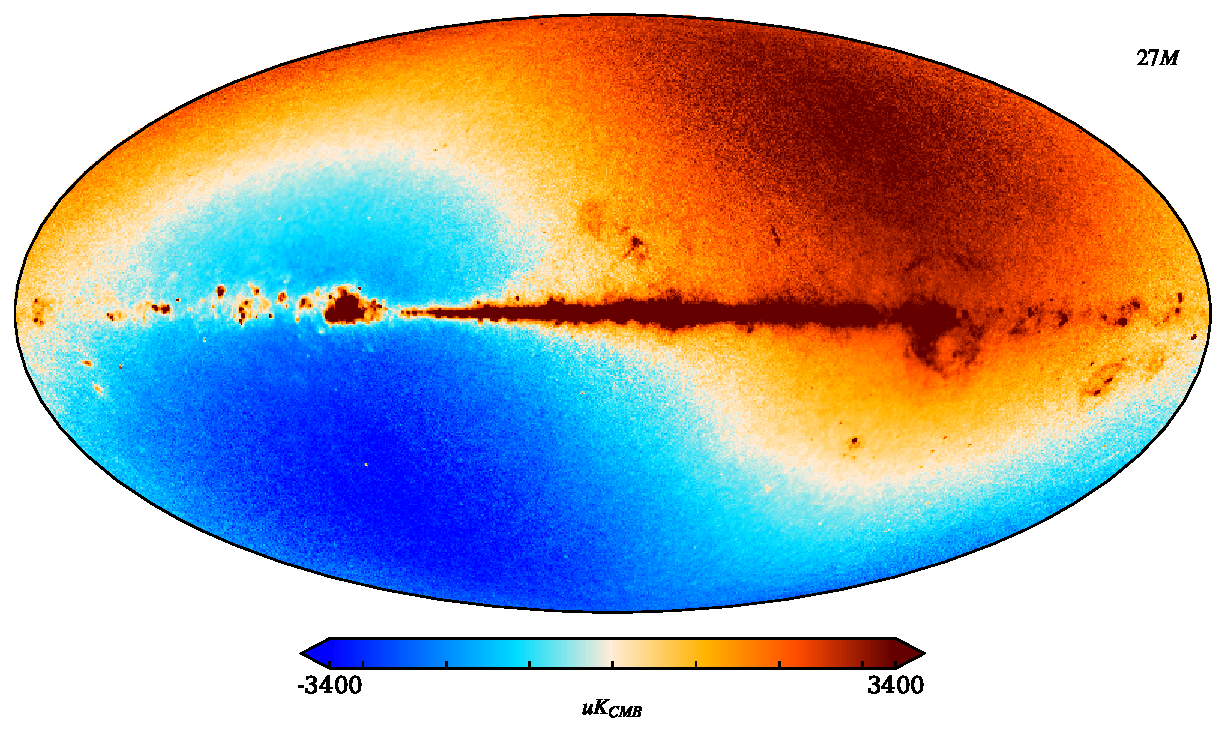
\includegraphics[width=0.49\textwidth]{figs/map_T_27M.pdf}
  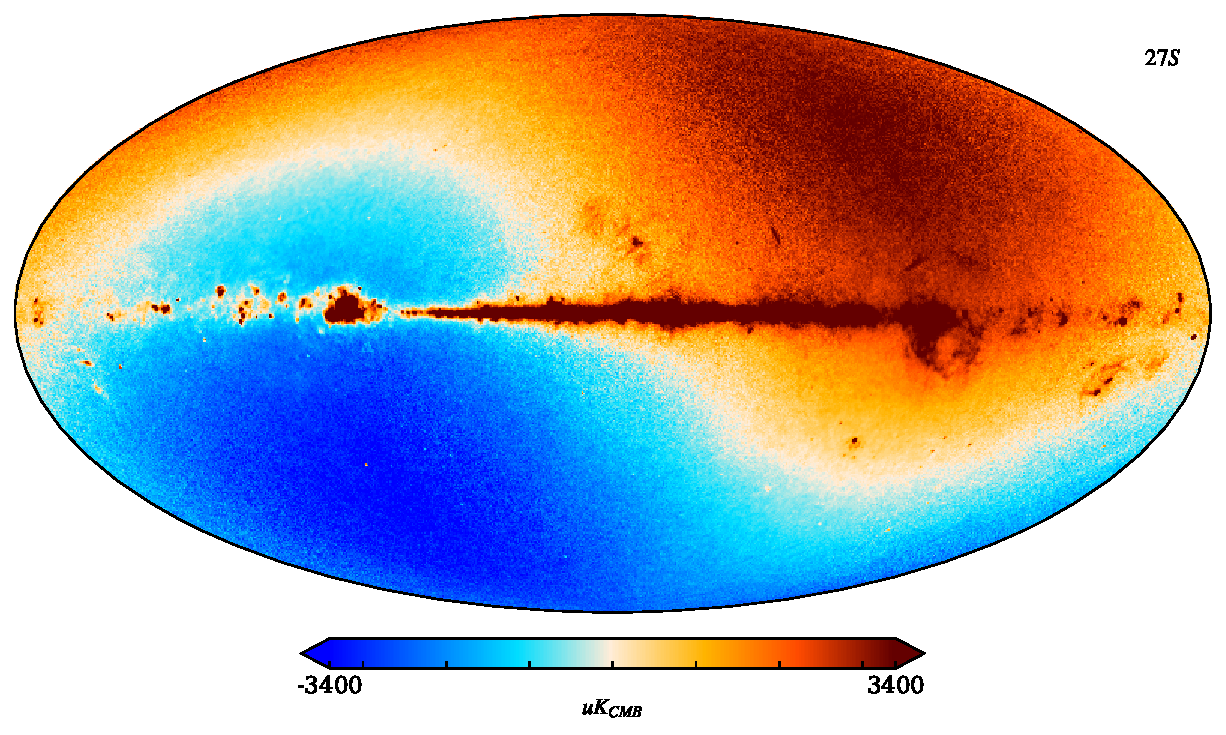
\includegraphics[width=0.49\textwidth]{figs/map_T_27S.pdf}\\
  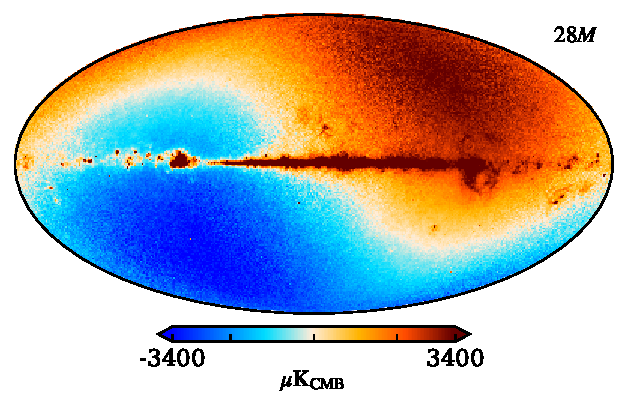
\includegraphics[width=0.49\textwidth]{figs/map_T_28M.pdf}
  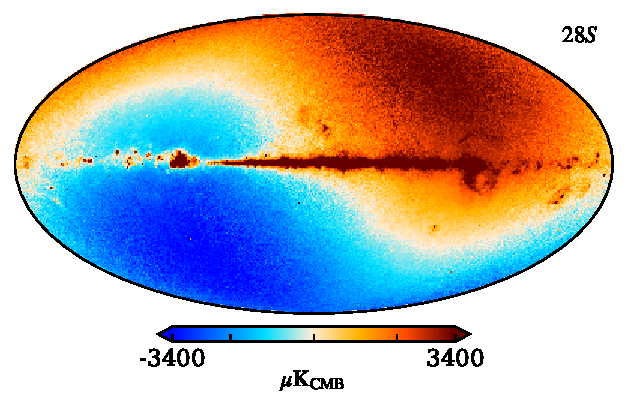
\includegraphics[width=0.49\textwidth]{figs/map_T_28S.pdf}\\
  %\includegraphics[width=0.5\columnwidth]{figs/cbar_temp.pdf}\\
  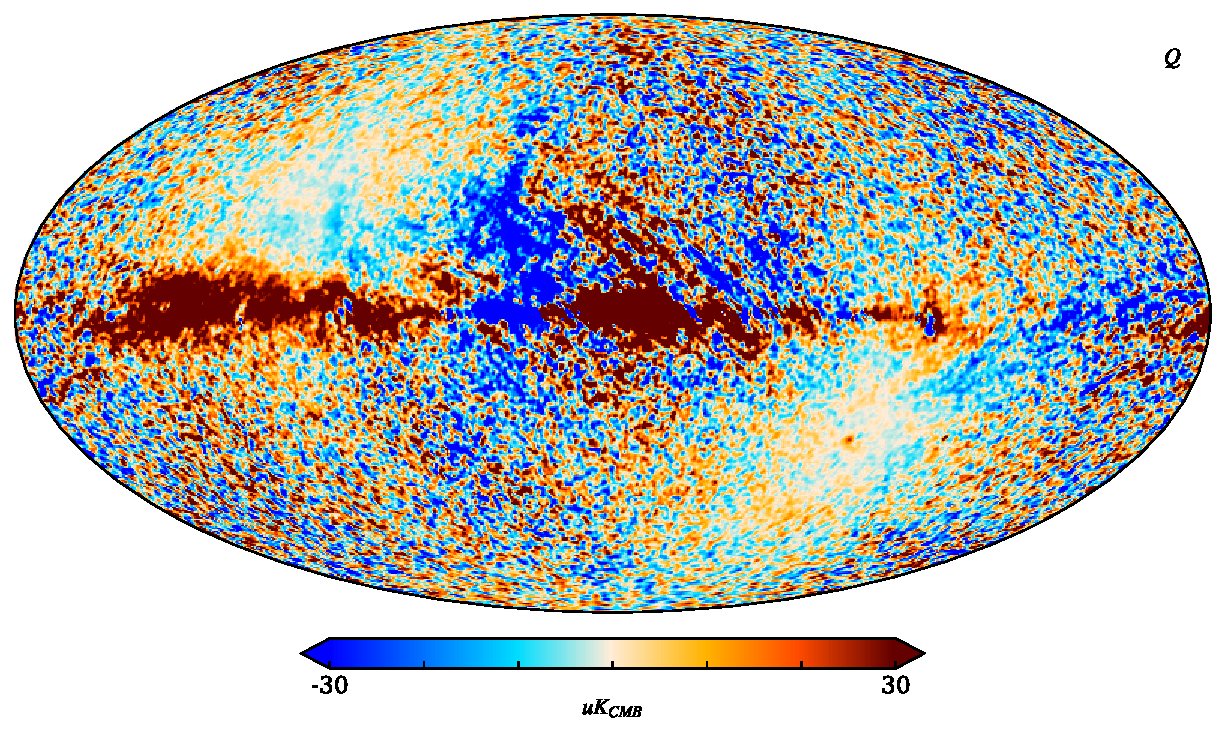
\includegraphics[width=0.49\textwidth]{figs/map_Q_badpol.pdf}
  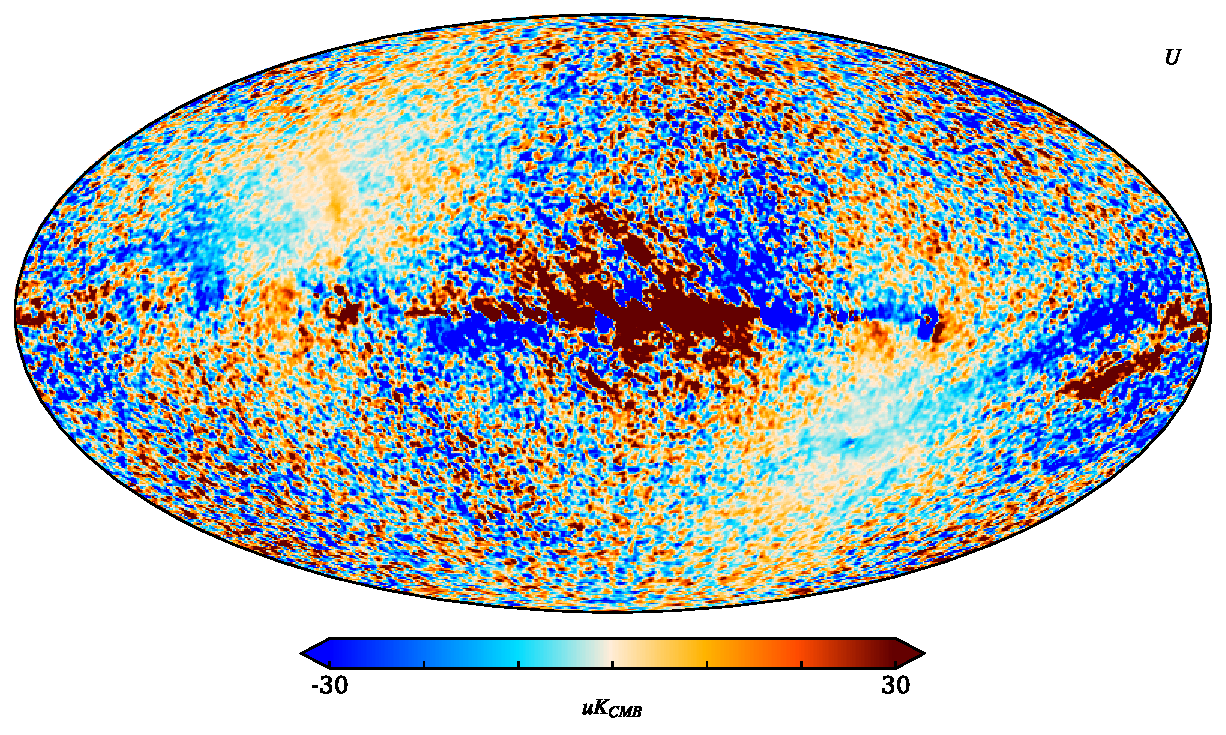
\includegraphics[width=0.49\textwidth]{figs/map_U_badpol.pdf}\\
    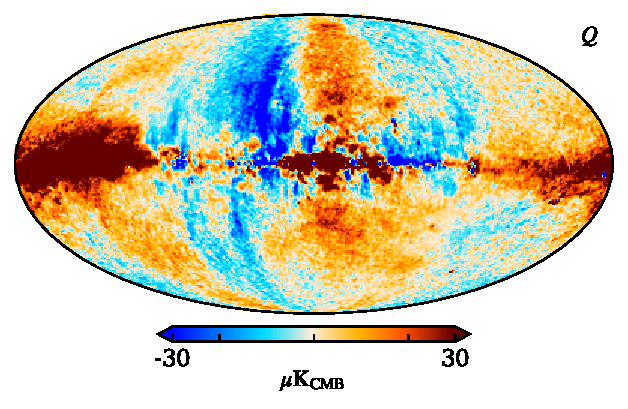
\includegraphics[width=0.49\textwidth]{figs/map_Q_binned.pdf}
  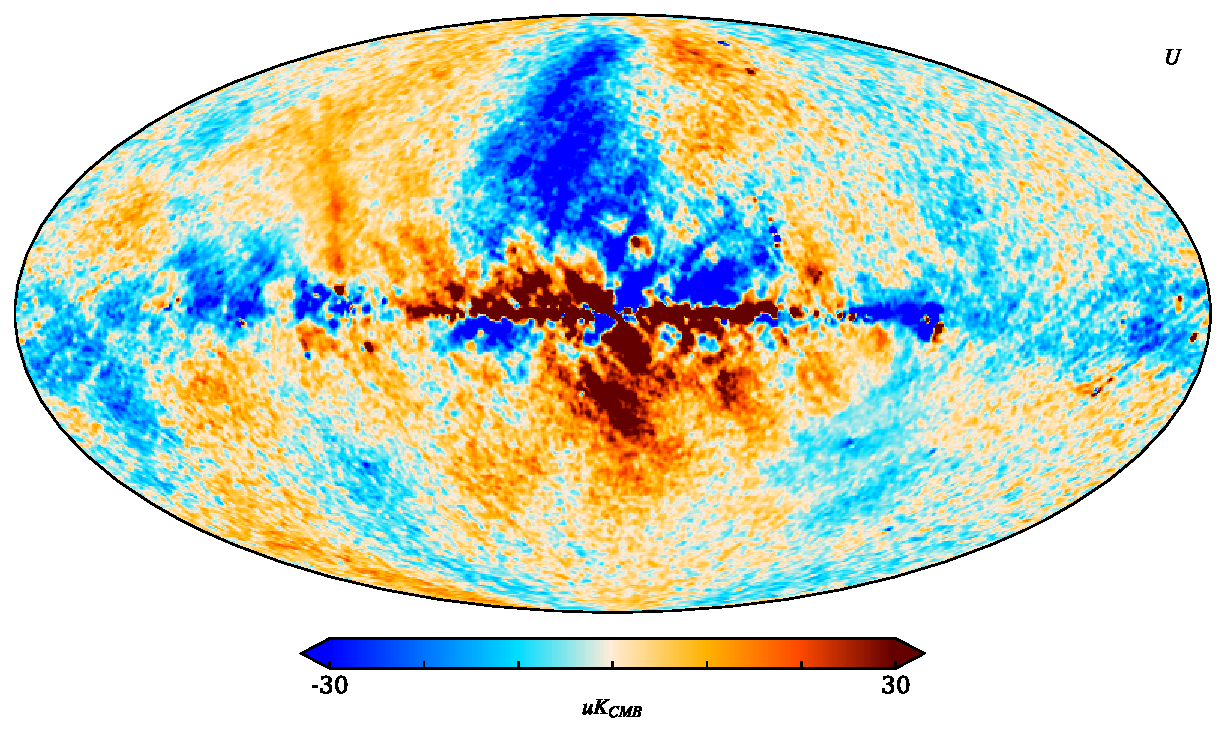
\includegraphics[width=0.49\textwidth]{figs/map_U_binned.pdf}\\
  %\includegraphics[width=0.5\columnwidth]{figs/cbar_pol.pdf}\\
  \caption{Temperature and polarization maps of the LFI 30 GHz data produced using n+2 mapmaking. The top four panels contain the temperature maps, and the third row contains the combined Q and U maps. The bottom row contains the Q and U maps produced from the traditional binned mapmaker where we invert the standard 3x3 matrix. \newline \newline \newline}
  \label{fig:maps}
\end{figure*}

\begin{figure*}
  \centering
  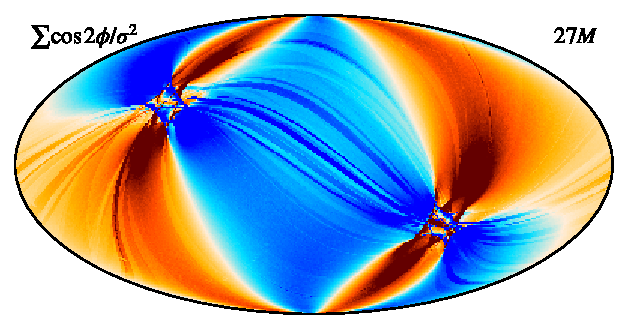
\includegraphics[width=0.49\textwidth]{figs/map_Q_polang27M.pdf}
  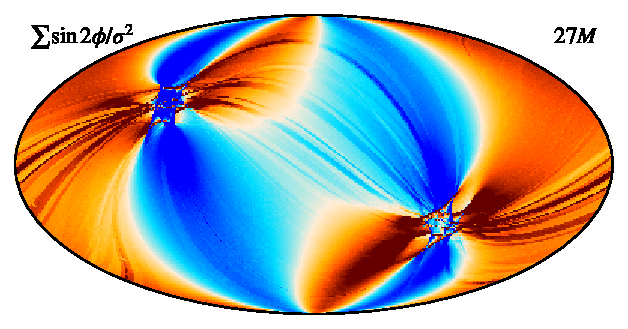
\includegraphics[width=0.49\textwidth]{figs/map_U_polang27M.pdf}\\
  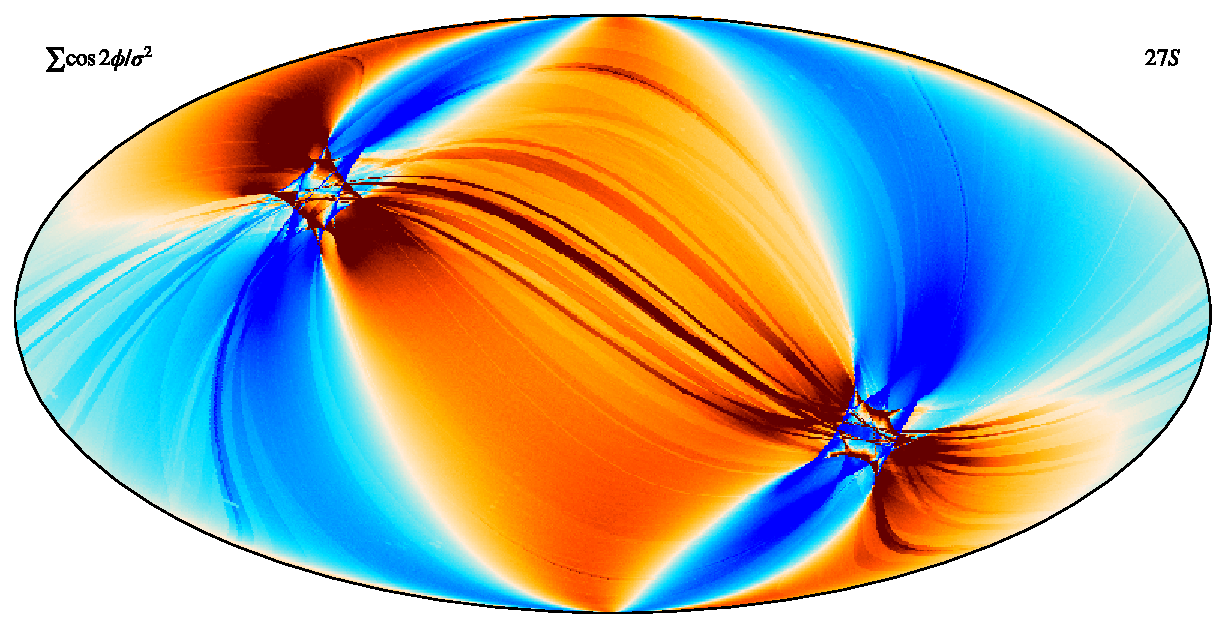
\includegraphics[width=0.49\textwidth]{figs/map_Q_polang27S.pdf}
  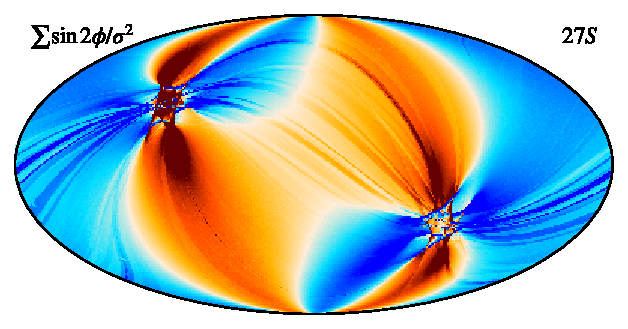
\includegraphics[width=0.49\textwidth]{figs/map_U_polang27S.pdf}\\
  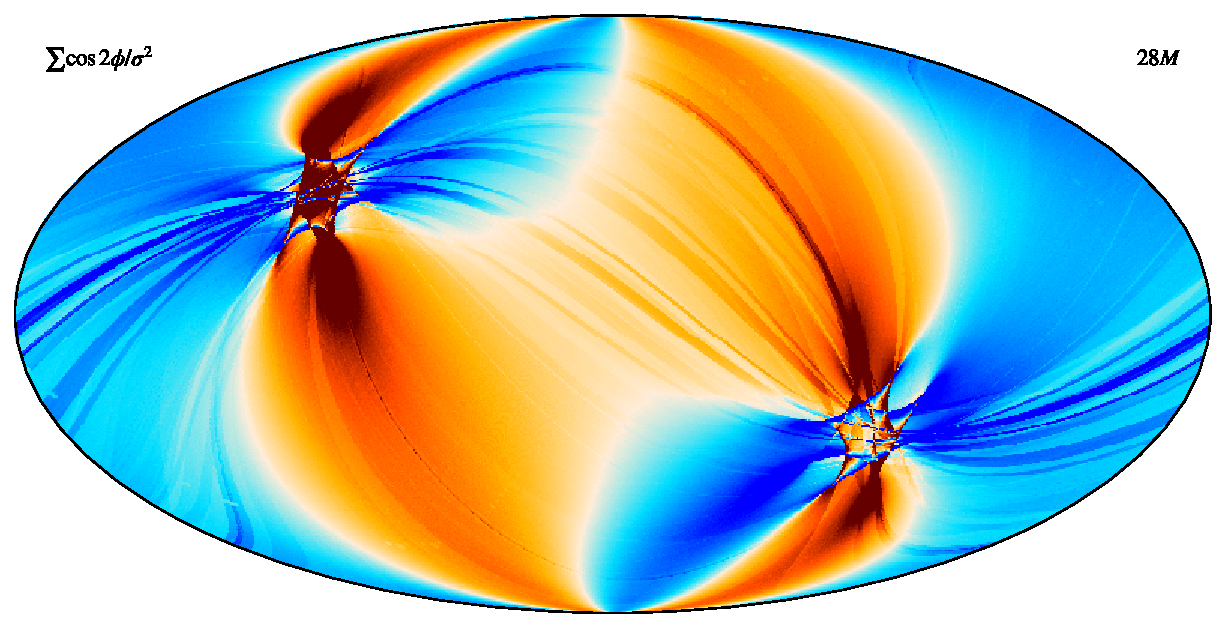
\includegraphics[width=0.49\textwidth]{figs/map_Q_polang28M.pdf}
  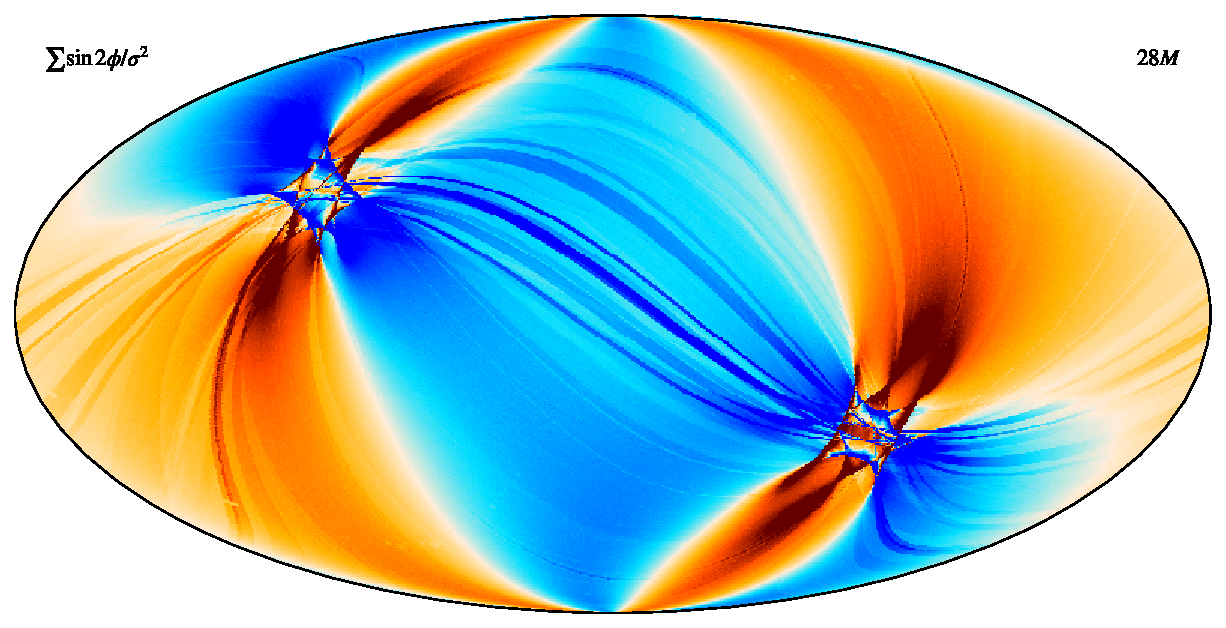
\includegraphics[width=0.49\textwidth]{figs/map_U_polang28M.pdf}\\
  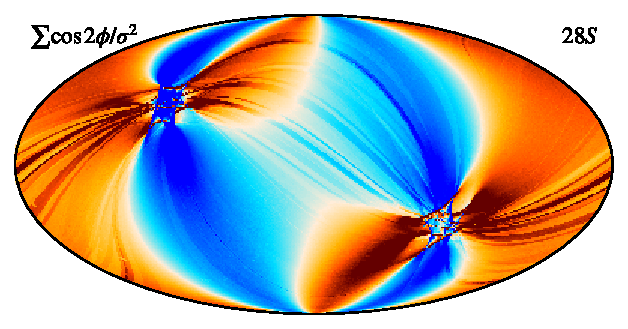
\includegraphics[width=0.49\textwidth]{figs/map_Q_polang28S.pdf}
  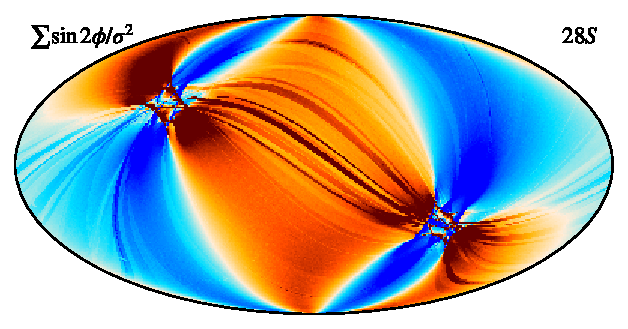
\includegraphics[width=0.49\textwidth]{figs/map_U_polang28S.pdf}\\
  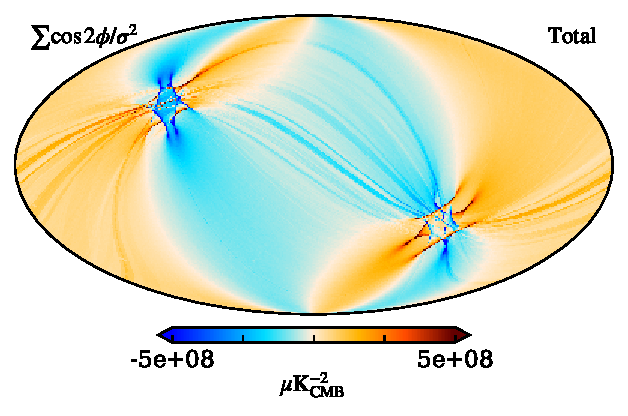
\includegraphics[width=0.49\textwidth]{figs/map_Q_polang_all.pdf}
  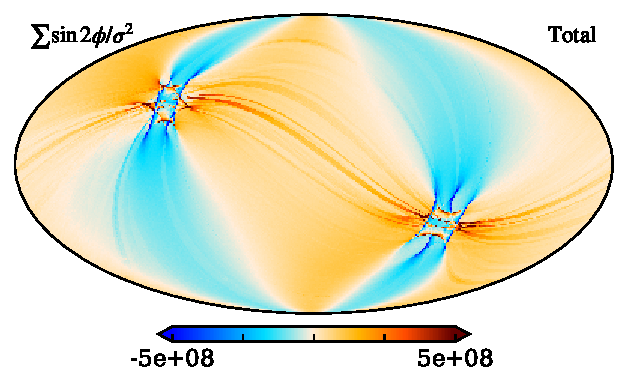
\includegraphics[width=0.49\textwidth]{figs/map_U_polang_all.pdf}\\
  %\includegraphics[width=0.5\columnwidth]{figs/cbar_pol.pdf}\\
  \caption{Polarization terms from the four 30GHz LFI detectors (rows 1-4) and the combined term used by the traditional binned mapmaker (bottom row). The left column is the Q term $(\frac{1}{\sigma})^2 cos2\phi$, and the right column is the U term, $(\frac{1}{\sigma})^2 sin2\phi$.}
  \label{fig:polangles}
\end{figure*}

\section{Mathematical Description}
\label{sec:mapmaking}

\begin{figure*}[!]
  \centering
  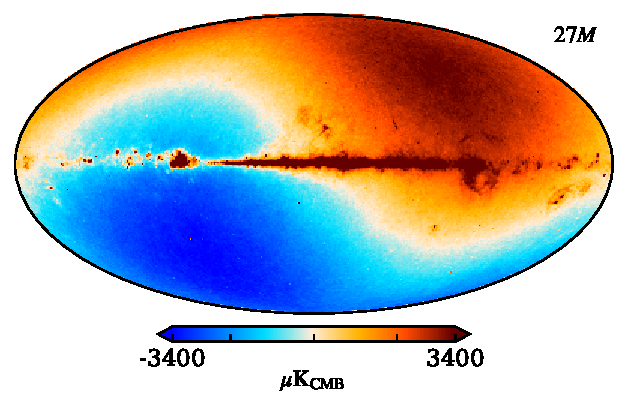
\includegraphics[width=0.49\textwidth]{figs/map_T_27M_depol.pdf}
  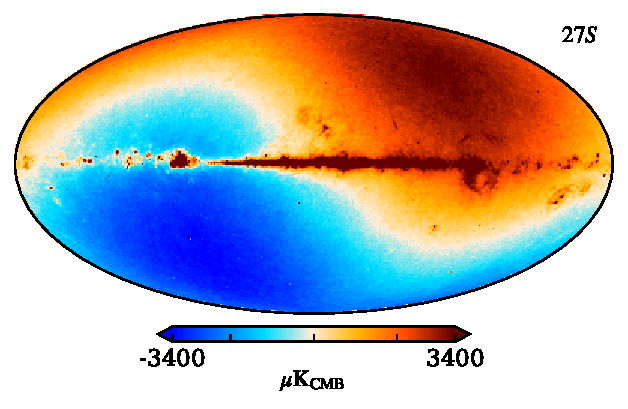
\includegraphics[width=0.49\textwidth]{figs/map_T_27S_depol.pdf}\\
  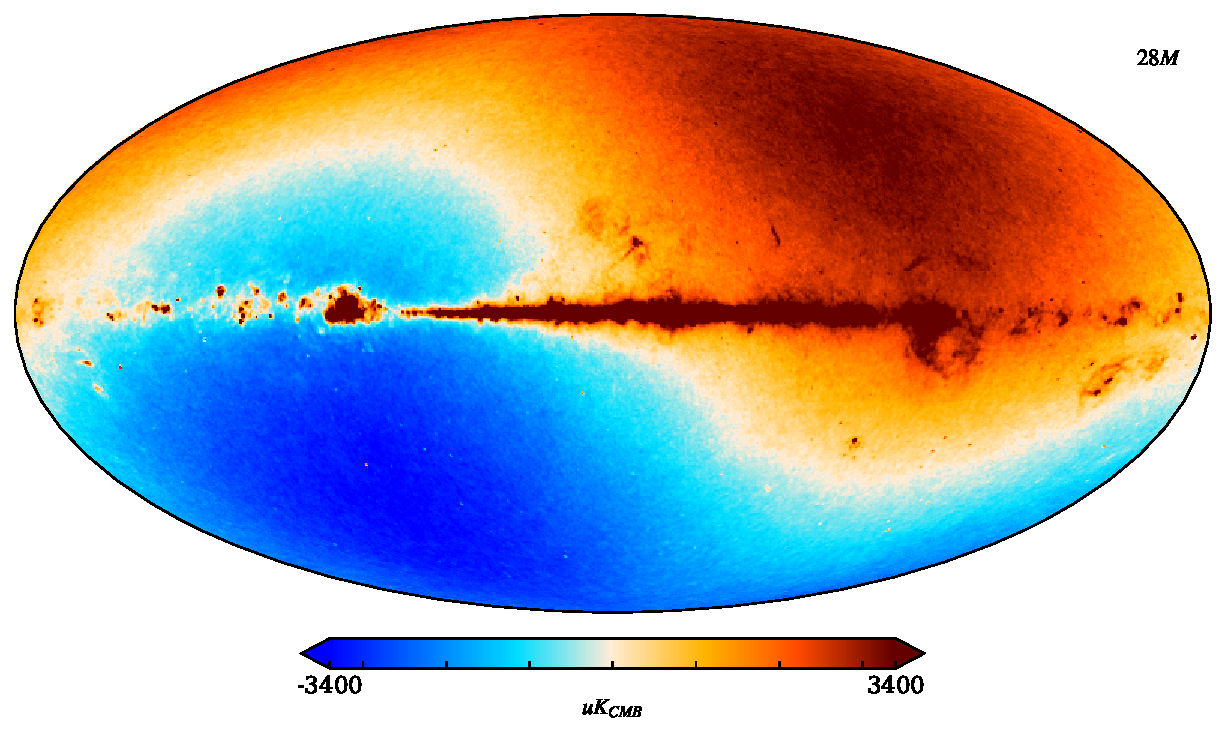
\includegraphics[width=0.49\textwidth]{figs/map_T_28M_depol.pdf}
  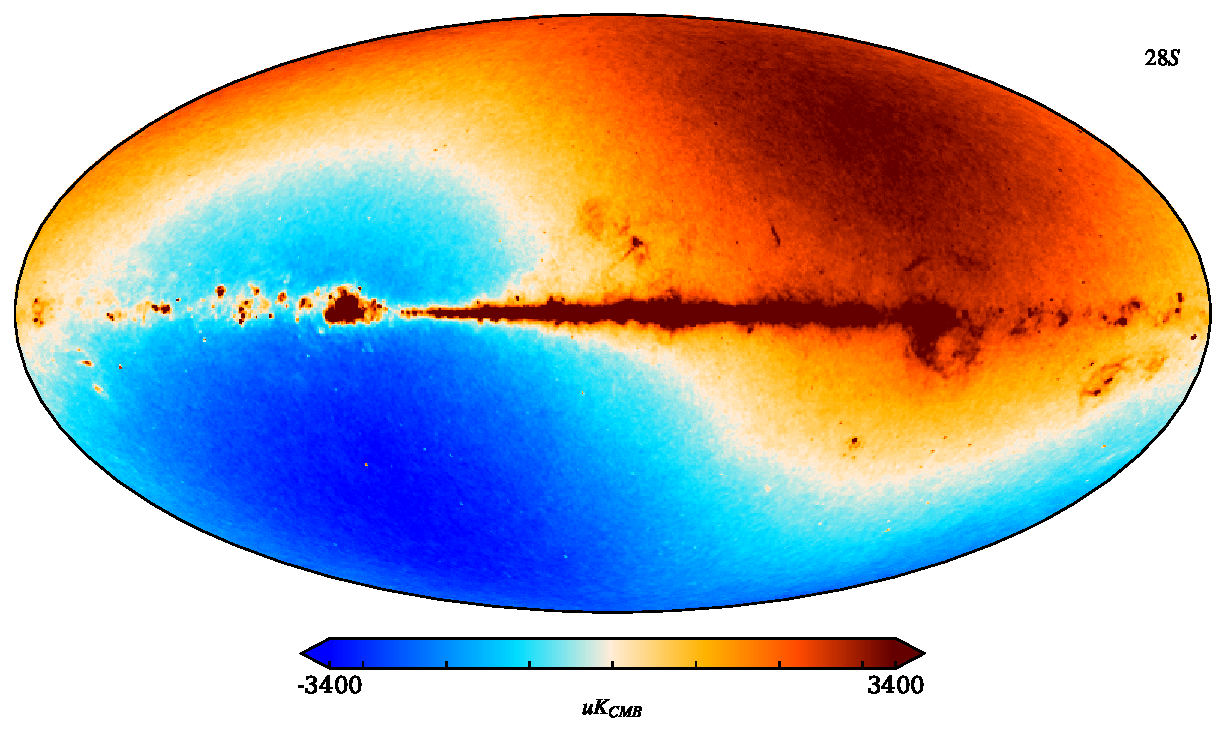
\includegraphics[width=0.49\textwidth]{figs/map_T_28S_depol.pdf}\\
  %\includegraphics[width=0.5\columnwidth]{figs/cbar_temp.pdf}\\
  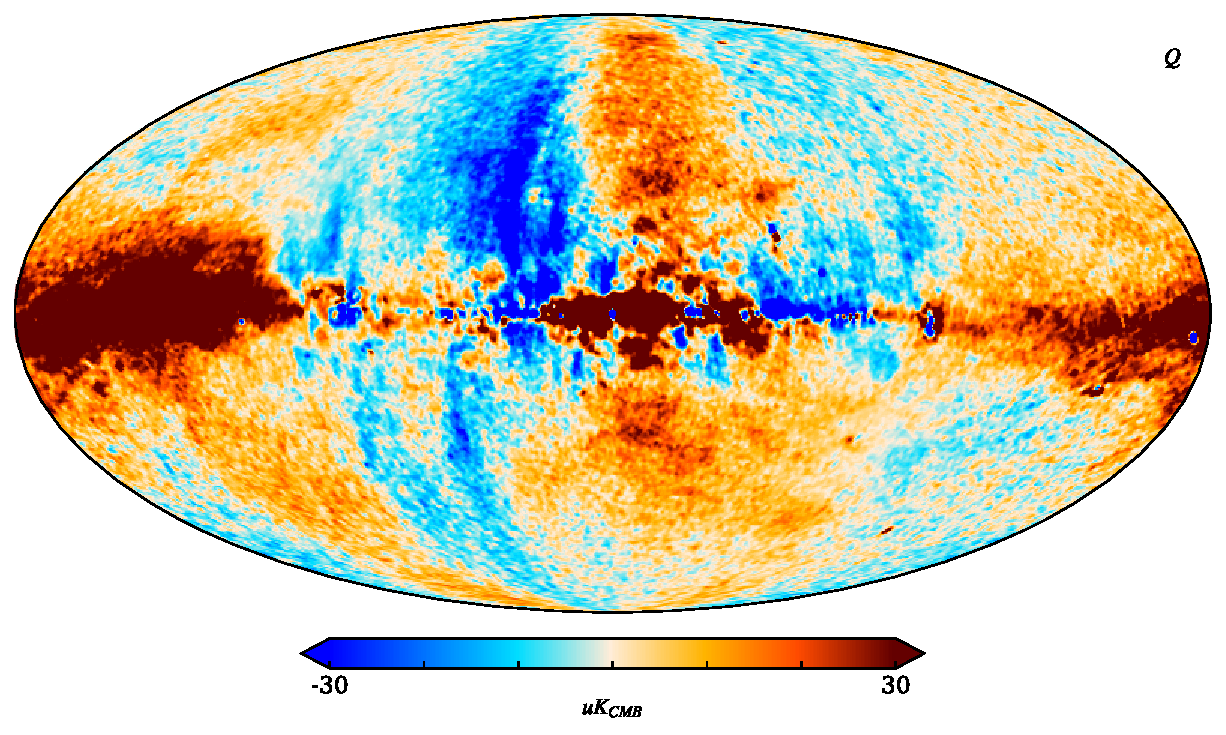
\includegraphics[width=0.49\textwidth]{figs/map_Q_depol.pdf}
  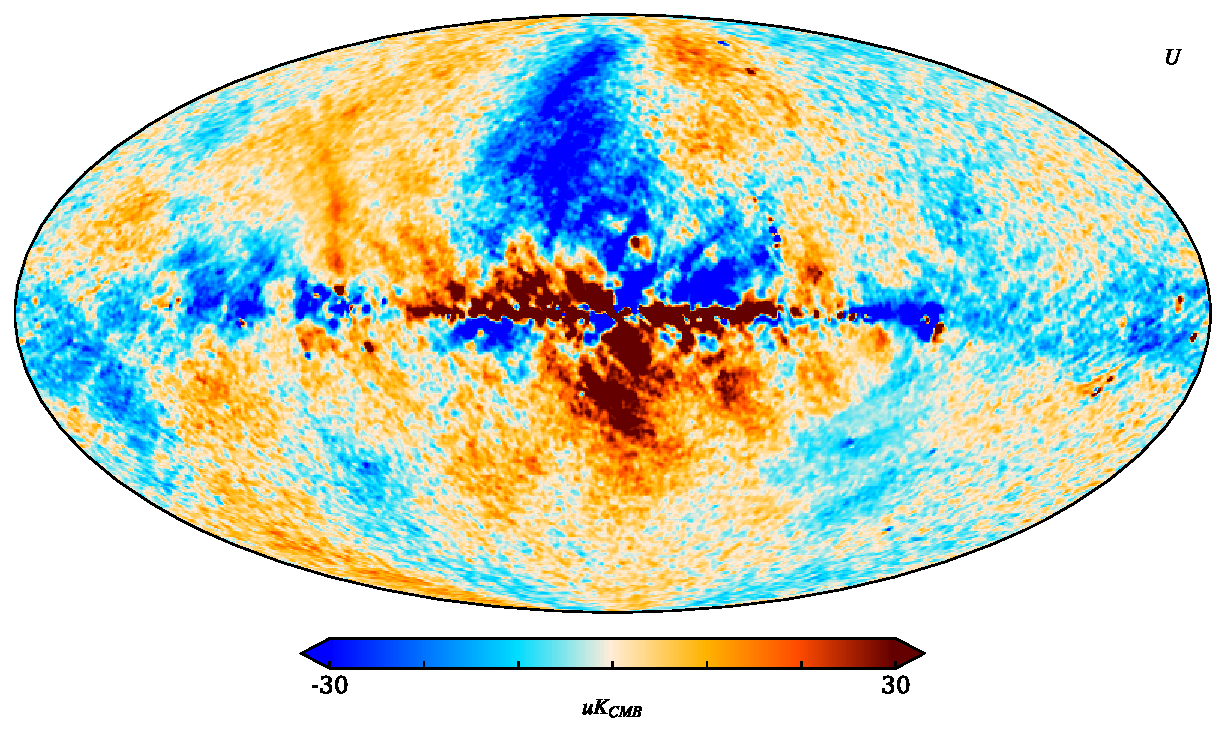
\includegraphics[width=0.49\textwidth]{figs/map_U_depol.pdf}\\
  %\includegraphics[width=0.5\columnwidth]{figs/cbar_pol.pdf}\\
  \caption{Temperature and polarization maps of the LFI 30 GHz data produced using depolarized n+2 mapmaking. The top four panels contain the temperature maps, and the bottom row contains the combined Q and U maps.}
  \label{fig:depolarized}
\end{figure*}

The mapmaking problem is often expressed in the literature as \citep[e.g.,][]{de_Gasperis_2005}
\begin{equation}
d_t = \A_{t,p}s_p + n_t,
\end{equation}
where $t$ and $p$ denote time sample and pixel, respectively; $d_t$ is the detector timestream; $\A$ is the pointing matrix; $s$ is the signal vector; and $n$ represents zero-mean instrumental Gaussian noise with covariance $\N$. In the case of $N+2$ mapmaking, we write $d_t$ as 
\begin{equation}
d_t = \begin{pmatrix}
d_t^1\\ d_t^2\\ \vdots \\ d_t^i\\
\end{pmatrix},
\end{equation}
where $i$ indexes detectors, while the sky signal for a single pixel, $s_p$, is written as
\begin{equation}
s_p = \begin{pmatrix}
I_{1,p}\\
I_{2,p}\\
\vdots\\
I_{i,p}\\
Q_p\\
U_p\\
\end{pmatrix}.
\end{equation}
This differs from the standard approach by allowing individual temperature maps per detector. Our data model for the timestream of a single detector $i$ then becomes
\begin{equation}
d_{i,p,t} = I_{i,p} + Q_p \cos2\phi_i(t) + U_p \sin2\phi_i(t).
\label{eq:datamodel}
\end{equation}
The $Q$ and $U$ terms are in this model common between all detectors, and thus independent of $i$.

Based on this model, we generalize the pointing matrix such that it maps the correct detector to the correct temperature map,
\begin{equation}
\A_{t,p} = \begin{pmatrix}
1 & 0 & \cdots & 0 & \cos2\phi_1 & \sin2\phi_1 \\
0 & 1 & \cdots & 0 & \cos2\phi_2 & \sin2\phi_2 \\
\vdots & \vdots & \ddots & \vdots & \vdots & \vdots \\
0 & 0 & \cdots & 1 & \cos2\phi_i & \sin2\phi_i \\
\end{pmatrix},
\end{equation}
where, for notational ease, we have dropped the explicit function of time for the polarization angles. The standard Generalized Least Squares (GLS) solution to the mapmaking equation is as usual given by
\begin{equation}
\tilde{s}_p = (\A^t \N^{-1}\A)^{-1} \A^t\N^{-1}d.
\label{eq:gls}
\end{equation}

\begin{figure*}
\begin{tabular}{B C C C}
& 27S & 28M & 28S\\
  
  27M & 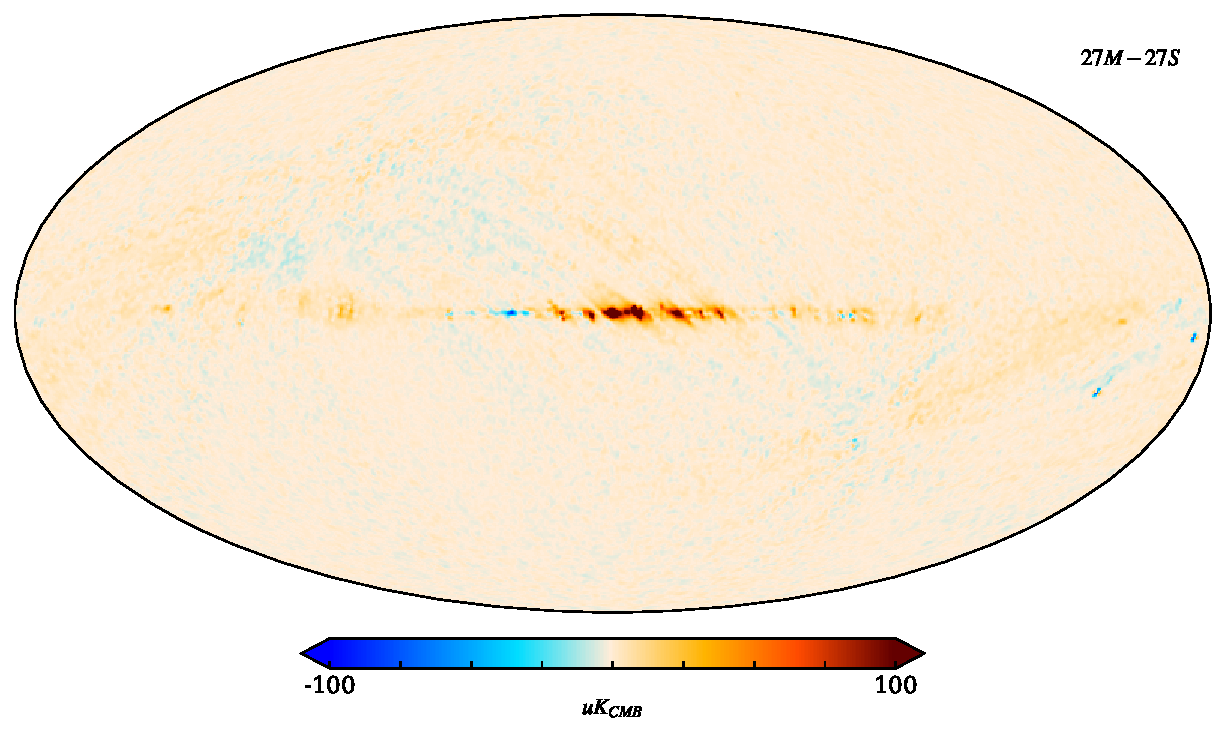
\includegraphics[width=0.31\textwidth]{figs/27M_minus_27S_depol.pdf} & 
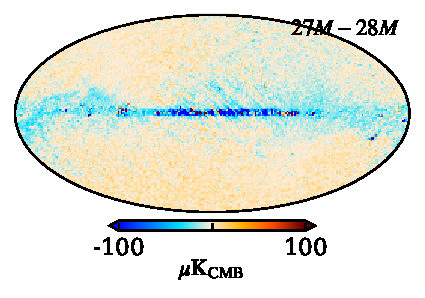
\includegraphics[width=0.31\textwidth]{figs/27M_minus_28M_depol.pdf} &
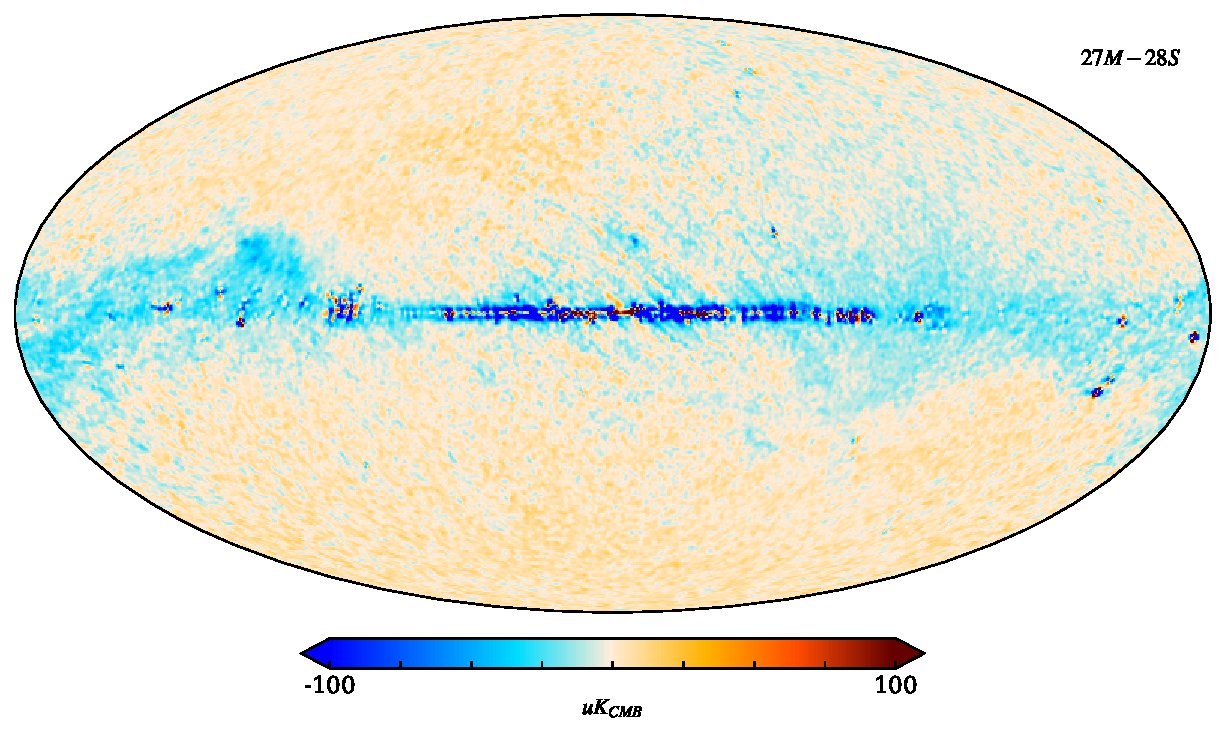
\includegraphics[width=0.31\textwidth]{figs/27M_minus_28S_depol.pdf}\\
 & \hspace{4.8cm } 27S & 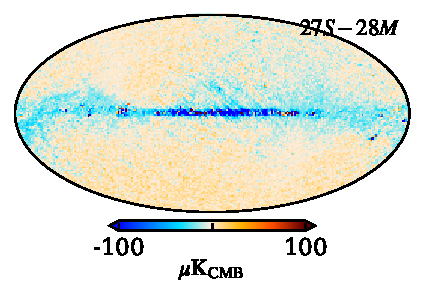
\includegraphics[width=0.31\textwidth]{figs/27S_minus_28M_depol.pdf} &
 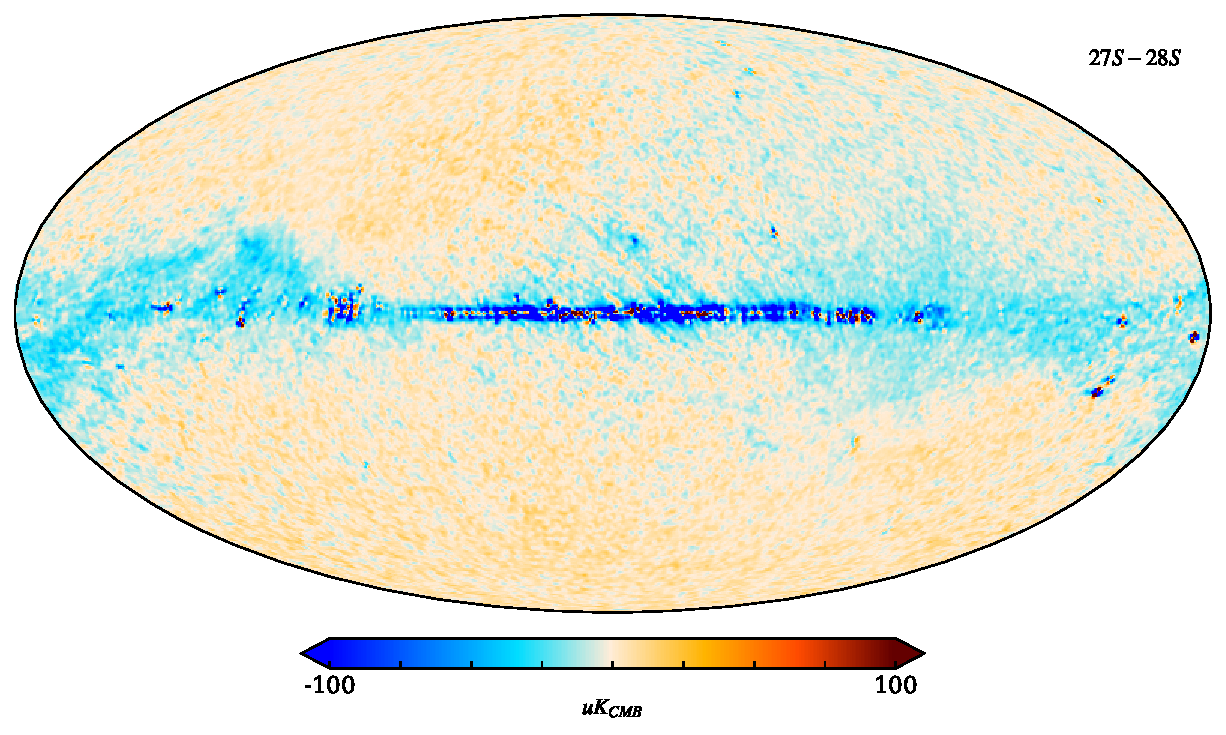
\includegraphics[width=0.31\textwidth]{figs/27S_minus_28S_depol.pdf}\\
 &     \caption{All 6 possible difference maps between the 30 Ghz detectors. } & \hspace{4.7cm } 28M  & 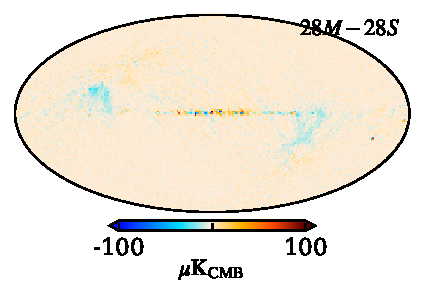
\includegraphics[width=0.31\textwidth]{figs/28M_minus_28S_depol.pdf} \\
  %\includegraphics[width=0.5\columnwidth]{figs/cbar_pol.pdf}\\
  \end{tabular}
\vspace{-0.75cm}
      \label{fig:bp_diffs}
\end{figure*}


During the mapmaking process, we must accumulate the quantity $\A^t\N^{-1}\A$. Assuming $\N$ to be diagonal and given by
\begin{equation}
N = \begin{pmatrix}
\sigma^2_1 & 0 & \cdots & 0 \\
0 & \sigma^2_2 & \cdots & 0 \\
\vdots & \vdots & \ddots & \vdots \\
0 & 0 & \cdots & \sigma^2_i \\
\end{pmatrix},
\end{equation}
this quantity expands into
\begin{equation*}
\begin{tiny}
\sum_t
\begin{pmatrix}
(\frac{1}{\sigma_1})^2 & 0 & \cdots &
(\frac{1}{\sigma_1})^2 \cos2\phi_1 & (\frac{1}{\sigma_1})^2 \sin2\phi_1 \\

0 & (\frac{1}{\sigma_2})^2 & \cdots &
(\frac{1}{\sigma_2})^2 \cos2\phi_2 & (\frac{1}{\sigma_2})^2 \sin2\phi_2 \\

\vdots & \vdots & \ddots & \vdots & \vdots \\

(\frac{1}{\sigma_1})^2 \cos2\phi_1 & (\frac{1}{\sigma_2})^2 \cos2\phi_2 & \cdots & 
\sum_{i} (\frac{\cos 2\phi_i}{\sigma_i})^2 & \sum_{i} \frac{\sin2\phi_t \cos2\phi_i}{\sigma_i^2}  \\

(\frac{1}{\sigma_1})^2 \sin2\phi_1 & (\frac{1}{\sigma_2})^2 \sin2\phi_2 & \cdots &
\sum_{i} \frac{\sin2\phi_i cos2\phi_i}{\sigma_i^2}  & \sum_{i} (\frac{ \sin 2\phi_i}{\sigma_i})^2
\\
\end{pmatrix}
\end{tiny}
\end{equation*}
for a given pixel, where the sum over $t$ represents the sum over all observation hitting a particular pixel $p$. Simultaneously, we can also accumulate the vector $\A^t\N^{-1}d$ which has the form
\begin{equation}
\sum_t
\begin{pmatrix}
\frac{d_{1}}{\sigma_1^2} \\
\frac{d_{2}}{\sigma_2^2}\\
\vdots\\
\frac{d_{i}}{\sigma_i^2}\\
\sum_i \frac{d_{i}}{\sigma_i^2} \cos2\phi_i\\
\sum_i \frac{d_{i}}{\sigma_i^2} \sin2\phi_i\\
\end{pmatrix}.
\end{equation}
Once these quantities are computed for all observations over the entire mission, it remains to simply invert the first matrix and front multiply the data vector to obtain the sky vector $\tilde{s}$, as described by Eq.~\ref{eq:gls}.


%Traditional polarized mapmaking for CMB experiments uses a matrix that looks like this (for a given timestep omitting all other columns):

%\begin{equation}
%M = \begin{pmatrix} 
%1          & cos(2\phi) & sin(2\phi)\\
%cos(2\phi) & cos^2(2\phi) & sin(2\phi) cos(2\phi) \\
%sin(2\phi) & sin(2\phi) cos(2\phi) & sin^2(2\phi) \\ 
%  \end{pmatrix}
%\end{equation}

%For n+2 mapmaking, we can generalize it to look like this

%\begin{equation}
%M = \begin{pmatrix} 
%\delta_d & 0 & \cdots  & \delta_d cos(2\phi) & \delta_d sin(2\phi)\\
%0 & \delta_d & \cdots  & \delta_d cos(2\phi) & \delta_d sin(2\phi)\\
%\vdots & \vdots & \ddots & \vdots & \vdots \\
%\delta_d cos(2\phi) & \delta_d cos(2\phi) & \cdots  & cos^2(2\phi) & sin(2\phi) cos(2\phi) \\
%\delta_d sin(2\phi) & \delta_d sin(2\phi) & \cdots & sin(2\phi) cos(2\phi) & sin^2(2\phi) \\ 
%  \end{pmatrix}
%\end{equation}

%where the delta function $\delta_d$ indicates which detector of your n detectors this particular sample belongs to.

%We also must define the map vector, which for n detectors looks like

\section{Application to Planck LFI}
\label{sec:lfi}

\begin{figure*}
  \centering
  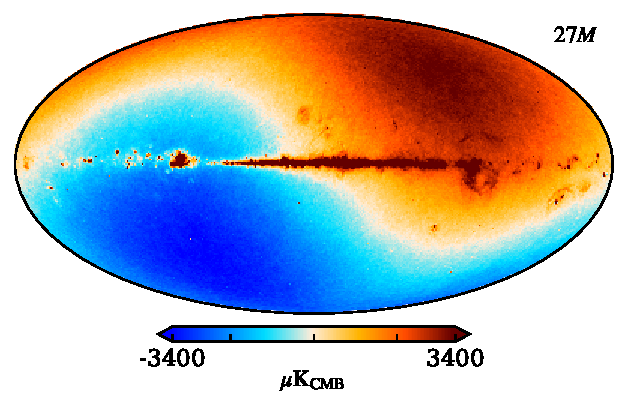
\includegraphics[width=0.49\textwidth]{figs/sim_T_27M.pdf}
  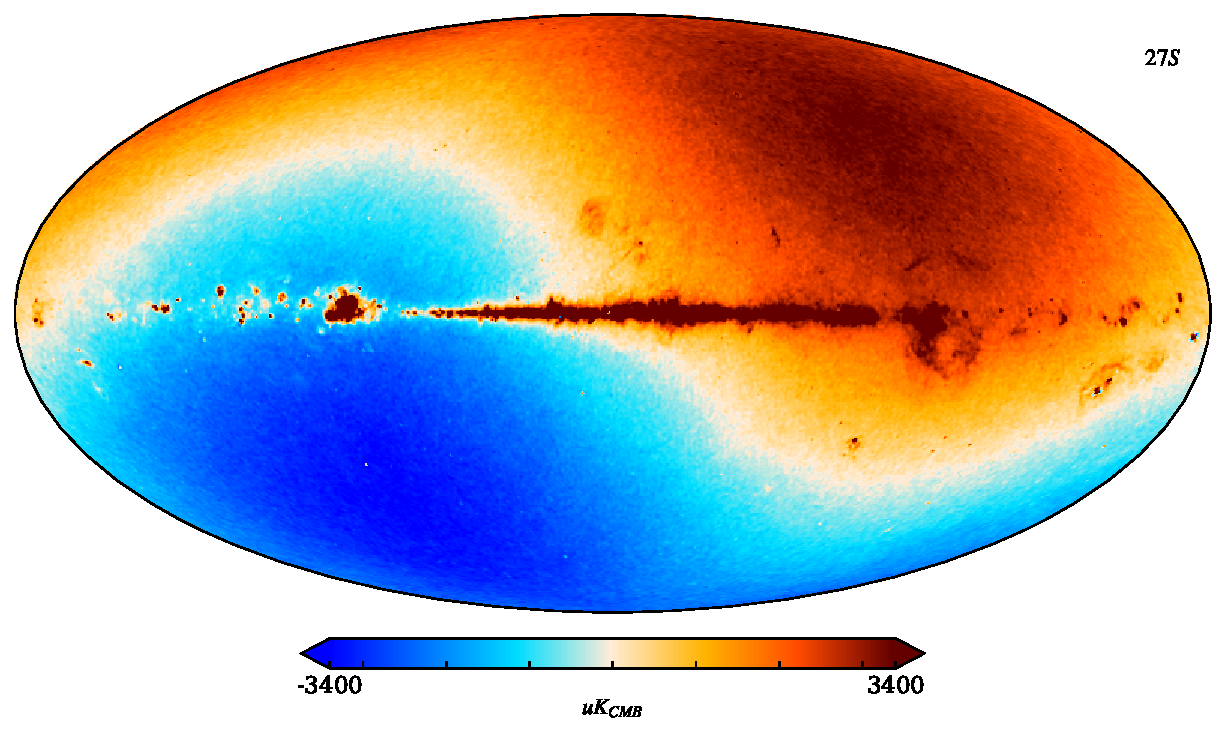
\includegraphics[width=0.49\textwidth]{figs/sim_T_27S.pdf}\\
  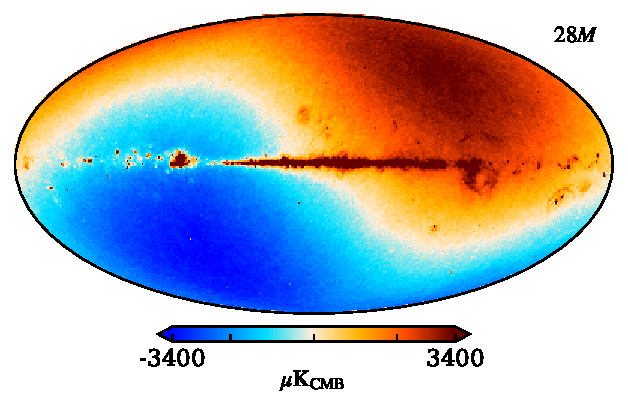
\includegraphics[width=0.49\textwidth]{figs/sim_T_28M.pdf}
  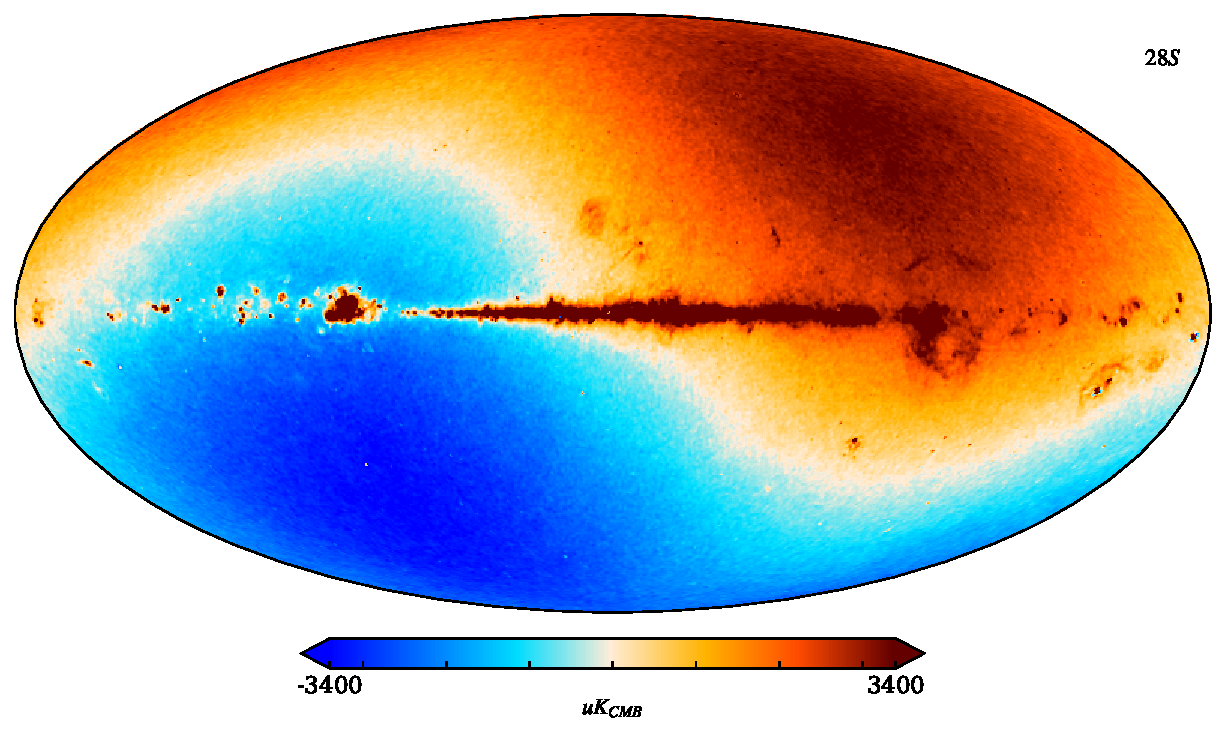
\includegraphics[width=0.49\textwidth]{figs/sim_T_28S.pdf}\\
  %\includegraphics[width=0.5\columnwidth]{figs/cbar_temp.pdf}\\
  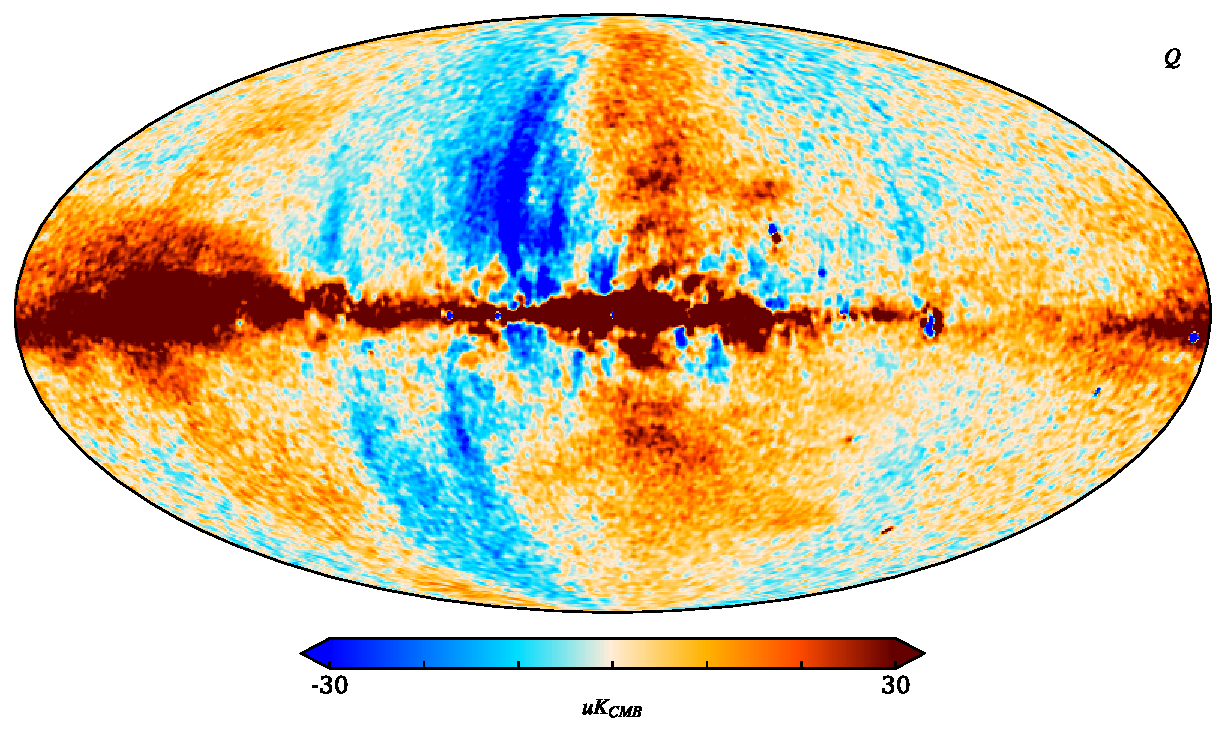
\includegraphics[width=0.49\textwidth]{figs/sim_Q.pdf}
  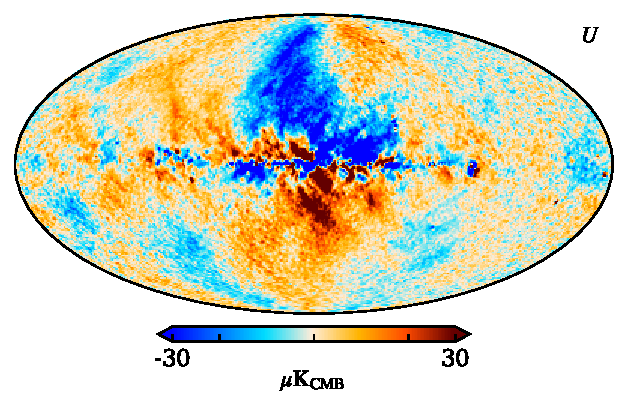
\includegraphics[width=0.49\textwidth]{figs/sim_U.pdf}\\
  %\includegraphics[width=0.5\columnwidth]{figs/cbar_pol.pdf}\\
  \caption{Simulated Temperature and polarization maps of the LFI 30 GHz data produced using n+2 mapmaking. The top four panels contain the temperature maps, and the bottom row contains the combined Q and U maps.}
  \label{fig:sim}
\end{figure*}


To demonstrate the effectiveness of this algorithm, we have applied it to the Planck LFI 30 GHz data, as analyzed in the commander3 pipeline by the BeyondPlanck and Cosmoglobe collaborations \citep{bp01, watts2023_dr1}. The raw TOD data has been processed as in those previous works, and the signal+white noise only data is fed to the n+2 mapmaker, instead of the full-frequency binned mapmaker that was presented in \citet{BP10}. 

As a brief summary of this algorithmic approach, we construct a complete model of the sky and instrument signals, which for LFI is given by:

\begin{equation}
  \begin{split}
    d_{j,t} = g_{j,t}&\tens{P}_{tp,j}\left[\tens{B}^{\mathrm{symm}}_{pp',j}\sum_{c}
      \tens{M}_{cj}(\beta_{p'}, \Delta_{\mathrm{bp}})a^c_{p'}  + \tens{B}^{\mathrm{asymm}}_{j,t}\left(\vec{s}^{\mathrm{orb}}_{j}  
      + \vec{s}^{\mathrm{fsl}}_{t}\right)\right] + \\
%    + s^{\mathrm{fsl}}_{j,t} + s^{\mathrm{mono}}_{j}\right] + \\
    + &n^{\mathrm{corr}}_{j,t} + n^{\mathrm{w}}_{j,t}.
  \end{split}
  \label{eq:todmodel}
\end{equation}

The details of the full model are discussed in \citep{bp01}, but the terms relevant to mapmaking are the pointing matrix $\tens{P}_{tp,j}$, the sky signal, which is the sum over sky components $\sum_{c} \tens{M}_{cj}(\beta_{p'}, \Delta_{\mathrm{bp}})a^c_{p'}$ and the white noise $n^{\mathrm{w}}_{j,t}$. The rest of the terms (like the sidelobes or correlated noise) are allowed by the Gibbs sampling algorithm \citep{gibbs} to be fixed, and thus can be treated as contaminants and removed during the time domain processing before the mapmaking occurs. 

This approach greatly simplifies the formal mapmaking process, as we do not need to mitigate correlated noise or other systematics during mapmaking, and can simply bin the TOD per pixel to beat down the white noise, using the approach detailed in section \ref{sec:mapmaking}.

Applying this to the four LFI 30 GHz detectors (27M, 27S, 28M, 28S), the nplus2 mapmaker produces 4 distinct temperature maps, as well as combined Q and U maps for the full 30 GHz frequency channel. These maps can be seen in Figure \ref{fig:maps}.

The bottom row of this figure shows the Q and U polarization maps produced from the traditional IQU mapmaker, which have been extensively verified by multiple implementations of the algorithm over many years \citep{lfi2013,lfi2015,lfi2018}. The failure of our N+2 polarization maps to resemble them is clearly a problem with this method that we investigate in the next section.

\subsection{Polarization Angle Coverage}

The root cause of these polarization issues seen in Fig. \ref{fig:maps} is the poor polarization angle coverage that LFI has, caused by its scan strategy. When the Planck mission was designed, it was highly optimized for temperature mapmaking and gain stability, which resulted in an approach when Planck scanned in great circles in ecliptic coordinates, modulated by a slow cycloidal procession to improve coverage at the ecliptic poles. \citep{planckScan} While this was effective at achieving a fairly uniform depth of coverage across the sky, it had some unfortunately consequences for polarization coverage.

Each Planck detector visits each pixel from the same angle of approach each time, with only a small variation in the polarization angle $\phi$. Without summing the different detectors together this results in a poorly conditioned matrix $A^tN^{-1}A$. This can be seen visually in Fig. \ref{fig:polangles}, where we plot the off-diagonal temperature-polarization cross terms ($(\frac{1}{\sigma_i})^2 cos2\phi_i$ and $(\frac{1}{\sigma_i})^2 sin2\phi_i$) for the four 30GHz detectors as well as for the full combined channel map. 

For an experiment with theoretically perfect polarization coverage, these maps should be consistent with zero, as the sine and cosine terms will cancel when averaged over the polarization angle $\phi$. The full frequency channel in the bottom row of Fig. \ref{fig:polangles} is almost an order of magnitude less than any of the individual detectors on their own and this discrepancy leads to poor condition number in the $A^t N^{-1}A$ matrix. The standard 3x3 case for a typical pixel has a condition number around 2, whereas the condition number for the N+2 case was on the order of 100. This means that we must unfortunately abandon this mathematically optimal procedure for real Planck data, and proceed with a reduced complexity case that can better handle this polarization coverage issue.

\section{Depolarized maps}
\label{sec:depol}

\begin{figure*}
  \centering
  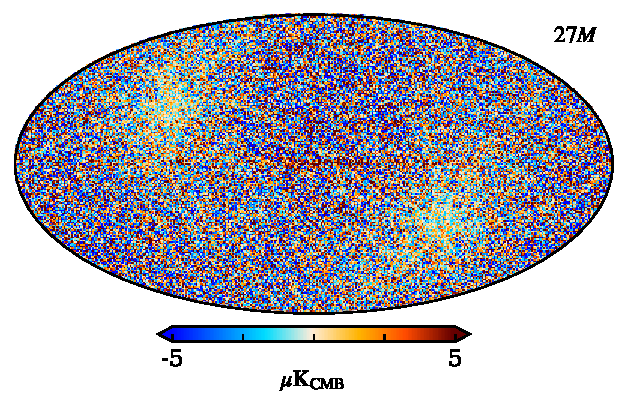
\includegraphics[width=0.49\textwidth]{figs/sim_diff_T_27M.pdf}
  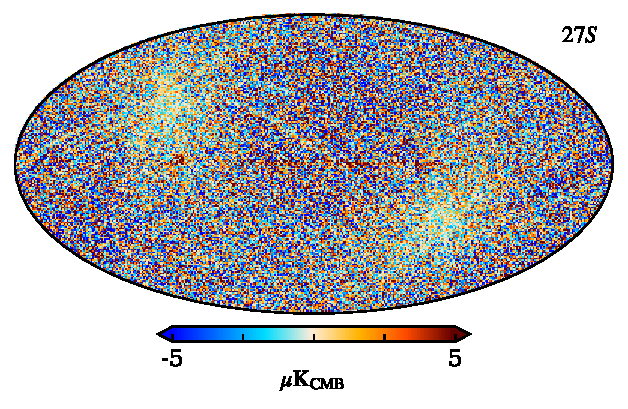
\includegraphics[width=0.49\textwidth]{figs/sim_diff_T_27S.pdf}\\
  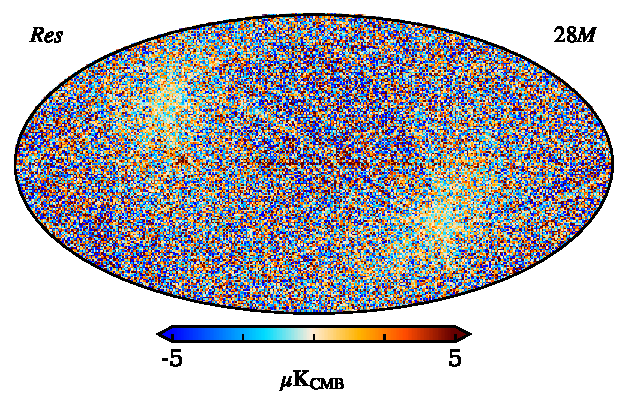
\includegraphics[width=0.49\textwidth]{figs/sim_diff_T_28M.pdf}
  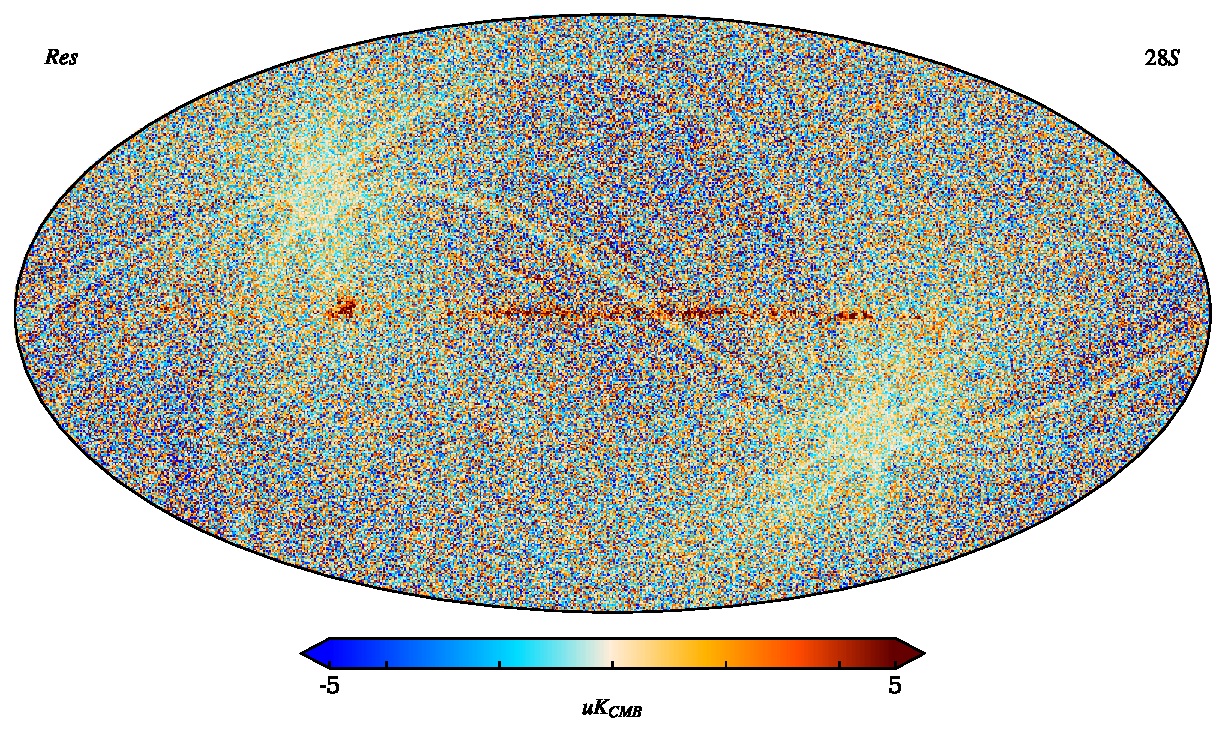
\includegraphics[width=0.49\textwidth]{figs/sim_diff_T_28S.pdf}\\
  %\includegraphics[width=0.5\columnwidth]{figs/cbar_temp.pdf}\\
  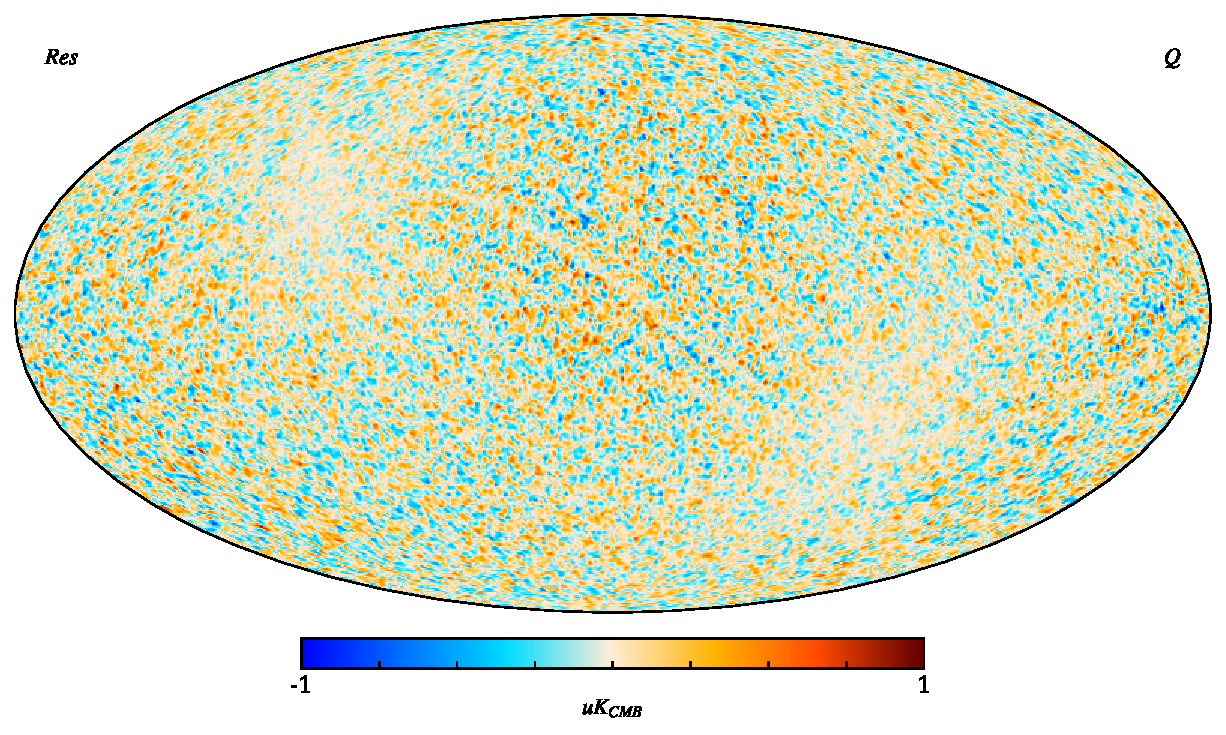
\includegraphics[width=0.49\textwidth]{figs/sim_diff_Q.pdf}
  \includegraphics[width=0.49\textwidth]{figs/sim_diff_U.pdf}\\
  %\includegraphics[width=0.5\columnwidth]{figs/cbar_pol.pdf}\\
  \caption{Input sky minus output maps for the simulated LFI 30GHz sky as generated using n+2 mapmaking in commander3. The top four panels contain the temperature maps, and the bottom row contains the combined Q and U maps.}
  \label{fig:sim_diff}
\end{figure*}

It is still possible, to simultaneously produce individual temperature maps and joint polarization maps in this case, albeit without all of the nice leakage-reducing properties of the ideal N+2 mapmaker. To generate our Q and U polarization maps in this case, we are forced to construct a traditional 3x3 $A^t N^{-1}A$ matrix, of the form

\begin{equation}
\begin{pmatrix}
(\frac{1}{\sigma})^2 &
(\frac{1}{\sigma})^2 cos2\phi_t & (\frac{1}{\sigma})^2 sin2\phi_t \\

(\frac{1}{\sigma})^2 cos2\phi_t & 
(\frac{cos 2\phi_t}{\sigma})^2 & (\frac{1}{\sigma})^2 sin2\phi_t cos2\phi_t \\

(\frac{1}{\sigma})^2 sin2\phi_t & 
(\frac{1}{\sigma})^2 sin2\phi_t cos2\phi_t &(\frac{ sin 2\phi_t}{\sigma})^2
\\
\end{pmatrix}
.
\end{equation}

Here, each entry includes contributions from every detector. We can then compute the GLS solution to Eq. \ref{eq:gls} and solve for our common sky signal vector 

\begin{equation}
S_p = \begin{pmatrix}
I_p\\
Q_p\\
U_p\\
\end{pmatrix}.
\end{equation}

Once we have derived $Q$ and $U$ for our pixel $p$, the temperature data as a function of time and pixel follows from the data model of eq. \ref{eq:datamodel}. 

\begin{equation}
T_{i,p} = d_{i,p,t} - Q_p \cos2\phi_t - U_p \sin2\phi_t.
\end{equation}


$Q_p$ and $U_p$ are given by the sky vector we solved for with the 3x3 case, and so to compute the depolarized temperature map for each detector we can simply perform a noise weighted sum over the time index $t$ for each pixel $p$. The quantities $\sum_t d_{i,p,t}/\sigma_t^2$, $\sum_t \cos2\phi_t/\sigma_t^2$ and $\sum_t \sin2\phi_t/\sigma_t^2$ have already been precomputed as elements of the N+2 mapmaking matrix, and so it is trivial to then solve for the depolarized temperature maps given the polarized components. 

These maps are shown in fig. \ref{fig:depolarized} for LFI 30GHz, and it is clear that this method produces a better result than that of the previous approach. The polarized maps are identical to those of the 3x3 binned mapmaker, but this approach maintains the additional advantage of producing the individual temperature maps.

Figure \ref{fig:bp_diffs} shows the 6 possible difference maps between these four temperature maps, smoothed to one degree to show their structure. These differences are largest in the galactic plane, where signals amplitudes are highest. We see that the 27M and 27S detectors predict similar skies, as do 28M and S, and the differences between 27 and 28 horns are more pronounced. Overall, the amplitudes are low enough to fall within the expected bounds.


\begin{figure*}
\begin{tabular}{B C C C}
& 27S & 28M & 28S\\
  27M & \includegraphics[width=0.30\textwidth]{figs/sim_27M_minus_27S.pdf} & 
\includegraphics[width=0.30\textwidth]{figs/sim_27M_minus_28M.pdf} &
\includegraphics[width=0.31\textwidth]{figs/sim_27M_minus_28S.pdf}\\
 & \hspace{4.8cm } 27S & \includegraphics[width=0.31\textwidth]{figs/sim_27S_minus_28M.pdf} &
 \includegraphics[width=0.31\textwidth]{figs/sim_27S_minus_28S.pdf}\\
 & \caption{All 6 possible difference maps between the simulated 30 GHz maps. } &  \hspace{4.7cm }  28M  & \includegraphics[width=0.31\textwidth]{figs/28M_minus_28S_depol.pdf} \\
  %\includegraphics[width=0.5\columnwidth]{figs/cbar_pol.pdf}\\
  \end{tabular}
\vspace{-0.75cm}
      \label{fig:bp_diffs}
\end{figure*}



\section{Well-conditioned N+2 mapmaking}
\label{sec:sim}


Despite being unable to apply N+2 mapmaking to Planck LFI, it remains an interesting option for other projects that have high temperature sensitivities but require joint polarization maps because of strange coverage, low signal-to-noise or systematics. In this section, we can demonstrate that the method works on a simulation of LFI 30 GHz where the polarization coverage problem present in real data has been mitigated.

Commander3 natively supports simulations, being able to generate noise and sky realizations within its sampling framework with ease \citep{BP04}. Here, we produce simulated timestreams to test the N+2 mapmaking algorithm. We start with the commander3 sky estimate for each channel, which is projected into the time domain through re-observation with the detector pointing and bandpasses. To mitigate LFI's poor polarization coverage, we instead use a simulated polarization angle, which is randomized across the sky for each detector, which should lead to the best possible coverage. White noise is then added to the simulated timesteam at a level consistent with the real 30 GHz data, and the resulting timestreams are then passed to the N+2 mapmaker. The resulting maps can be seen in Figure \ref{fig:sim}.

We can compare these output maps to the input sky signal used to produce them, to see if there are any discrepancies introduced by the N+2 mapmaking process. These difference maps can be seen in Figure \ref{fig:sim_diff}. They show some small discrepancies along the galactic plane in temperature caused by a lack of bandpass modelling in the simulation, a feature that was see with other mapmaker as well. The rest of the sky and the polarization maps are consistent with noise, leading us to conclude that this N+2 algorythm was working as intended.

Figure \ref{fig:sim_bp_diffs} shows the difference maps between each of our simulated temperature maps. Here, we see clear imprints of bandpass differences between each channel. Each difference map A minus B clearly shows an imprint of the galactic center, red if bandpass A is lower than bandpass B, and blue if B is lower than A. This sign depends on the dominant foreground in the galaxy, which at 30 GHz is synchrotron which is stronger at lower frequencies. These bandpass differences are precisely the effects that we intended to capture in the separate temperature maps using this approach, so it is no surprise that we detect them here.



\subsection{Bandpass Leakage Mitigation}

The main advantages of the N+2 mapmaker are twofold: firstly, the separation of the temperature maps for each detector improves our ability to perform component separation in the case of differing bandpasses, and secondly that it helps mitigate T to P leakage caused by bandpass differences. In Figure \ref{fig:leak}, we demonstrate this second benefit of N+2 mapmaking. 

\begin{figure}[]
\includegraphics[width=\linewidth]{figs/map_Q_leak_comp.pdf}\\
\includegraphics[width=\linewidth]{figs/map_Q_leak_nplus2_comp.pdf}
\caption{Comparison of T to P leakage from binned mapmaking (top) and N+2 mapmaking (bottom). Note the order of magnitude difference in the colour scales.}
\label{fig:leak}
\end{figure}

In our simulation pipeline, we now inject an artificial offset signal into one of the four 30 GHz detectors, with an amplitude of 1 mK. This is an crude representation of an offset due to a bandpass mismatch between detectors, but it serves well enough to illustrate this point. The signal is completely unpolarized, being added to each measurement uniformly, but due to its large amplitude, temperature to polarization leakage can still be a problem. The top of fig. \ref{fig:leak} is the Q polarization leakage generated when these detectors are combined using traditional mapmaking with a 3x3 pointing matrix $A$. This is calculated by subtracting the simulated map from one generated without this additional temperature signal. The bottom panel shows the leakage from the same procedure performed for the N+2 mapmaker. The amplitude of the polarization leakage in this second case is now more than six orders of magnitude fainter, because the mapmaker is able to properly distinguish temperature differences between detectors from true polarized signal. 

\section{Conclusions and Future Plans}
\label{sec:conclusions}

N+2 mapmaking is a novel method of extracting temperature and polarization maps from CMB timestreams. It is especially useful in cases with strong signal-to-noise in intensity but that still require combined polarization maps. Using this method, it is possible to separate out the effects of bandpass discrepancies between different detectors, improving our ability to perform component separation, as well as greatly mitigating Temperature to Polarization leakage. 

In this paper, we developed the GLS solution for N+2 mapmaking problem, based on existing mapmaking approaches. We apply that formalism to the Planck LFI 30 GHz data within the Commander3 framework, producing independent temperature maps at the same time as combined polarization maps. These maps are unfortunately noise and leakage dominated, due to the poor intrinsic polarization coverage of each individual LFI detector. To mitigate this, we construct a new formalism, de-polarized N+2 mapmaking, which can still produce individual temperature maps for component separation but is unable to mitigate bandpass leakage in the polarization maps. 

Finally, to demonstrate the effectiveness of the original concept of N+2 mapmaking, we apply it to simulated LFI 30 GHz data, where we randomize the polarization angles for each detector, greatly improving the polarization coverage. With this better coverage, we are able to test this N+2 mapmaking approach, and show that it produces maps that match the input simulations well. We also demonstrate the effectiveness of this approach at mitigating T to P leakage caused by simulated bandpass mismatches in the data. 

The N+2 mapmaking algorithm was developed to be applied to Planck HFI, where leakage and CO lines are important effects to model and correct for. The OpenHFI initiative aims to re-analyze HFI in a Bayesian end-to-end framework, and this work marks the first new methodology that has been developed for that purpose. The next steps will be to integrate the N+2 mapmaker into an iterative CG solver to simultaneously estimate the maps and HFI's filter transfer function, similar to what was done in \cite{artem}. Once developed, this re-analysis will provide the most consistent Planck HFI maps to the community, and this paper represents the first step in the process.

\begin{acknowledgements}
 The current work has received funding from the European
  Union’s Horizon 2020 research and innovation programme under grant
  agreement numbers 819478 (ERC; \textsc{Cosmoglobe}) and 772253 (ERC;
  \textsc{bits2cosmology}). Some of the results in this paper have been derived using the HEALPix \citep{healpix} package.
  We acknowledge the use of the Legacy Archive for Microwave Background Data
  Analysis (LAMBDA), part of the High Energy Astrophysics Science Archive Center
  (HEASARC). HEASARC/LAMBDA is a service of the Astrophysics Science Division at
  the NASA Goddard Space Flight Center.  
\end{acknowledgements}


%-------------------------------------------------------------
%                                       Table with references 
%-------------------------------------------------------------
%

\bibliographystyle{aa}
\bibliography{references, ../../common/CG_bibliography}
\end{document}
%%%% End of aa.dem
